% % Класс документа пока не окончательный, сильно сомневаюсь, что article лучший
\documentclass[a4paper,12pt]{extarticle} 
% Подключаем шрифты,кодировки,русские переносы
\usepackage{cmap}
% подключается пакет, позволяющий улучшить вид пдф документа(как я понял)
\usepackage[T2A]{fontenc}
\usepackage[utf8x]{inputenc}
% подключаем кодировку шрифтов для вносимых файлов
\usepackage[main=russian,english]{babel}
% подключаем перенос и распознование слов, русский в приоритете
\usepackage{indentfirst}
% Отступ в начале абзаца
\usepackage{
	amssymb,
	amsfonts,
	amsmath,
}
% Пакеты американского математ. сообщества, красивый вид формул и текста внутри
\usepackage{
	wrapfig,
	graphicx,
	caption,
	subcaption,
	tikz,
}
% Обтекаемые объекты, рисунки, подписи и прочее
\usepackage{
	pgfplotstable,
	pgfplots,
	booktabs,
	colortbl,
	array
}
\pgfplotsset{compat=newest}
% таблицы, графики

\usepackage{xcolor}
\usepackage[unicode]{hyperref}

 % Цвета для гиперссылок
\definecolor{linkcolor}{HTML}{000000} % цвет ссылок
\definecolor{urlcolor}{HTML}{799B03} % цвет гиперссылок
\hypersetup{pdfstartview=FitH,  linkcolor=linkcolor,urlcolor=urlcolor, colorlinks=true}

\usepackage{geometry}
\usepackage{fancyhdr}
% границы, контитулы, и прочее


\geometry
	{
	left=2.2cm,
	right=2.2cm,
	bottom=2cm,
	top=2cm,
	}
% границы документа

\usepackage{setspace}
% убирает гигантские размеры оглавления
\linespread{1.3}
% междустрочный интервал

\pagestyle{fancy}
\fancyhead{}
% пустая шапка контитула
\fancyhead[R]{\authors}
% На правой стороне страницы авторы и науч.рук.
\fancyhead[L]{\shortlabname}
 % Слева название лабы
\fancyfoot{}
\fancyfoot[C]{\thepage}
% номер страницы снизу по середине
\renewcommand{\contentsname}{Оглавление}
% переводим на русский язык оглавление
\usepackage{secdot}
\sectiondot{subsection}
% Ставит злосчастные точки в главах, ибо не по госту
% Преамбула почти слизана у Федора Сарафанова https://github.com/FedorSarafanov/RLC/blob/master/text/diss.tex

% 	\def\authors{Есюнин М.В., Есюнин Д.В.}
% 	\def\labname{Частотный модем}
% 	\def\sciadviser{Земнюков Н.Е.}
% 	\def\shortlabname{Частотный модем}
% \usepackage{float}
% \usepackage{amsthm}
% \usepackage{misccorr} % в заголовках появляется точка, но при ссылке на них ее нет
% % \usepackage[usenames,dvipsnames]{color}
% % \hypersetup{%
% %     pdfborder = {0 0 0}
% % }
% \usepackage{makecell,multirow} 
% \usepackage{ulem}
% \begin{document}
% \begin{titlepage}

\begin{center}

	\textsc{Нижегородский государственный университет имени Н.\,И. Лобачевского}
	\vskip 4pt \hrule \vskip 8pt
	\textsc{Радиофизический факультет}

	\vfill

	{\Large\labname}

\end{center}

\vfill

\begin{flushright}
	{Работу выполнили студенты\\ \authors\\ 430 группы\\ \vskip 14pt преподаватель:\\ \sciadviser}
\end{flushright}

\vfill

\begin{center}
	Нижний Новгород, \the\year
\end{center}

\end{titlepage}
% % \renewcommand{\vec}{\mathbf}

% \renewcommand{\phi}{\varphi}
% \renewcommand{\hat}{\widehat}

% \tableofcontents

% \newpage
% \sloppy
\documentclass[a4paper,12pt]{article}

\usepackage{cmap}
\usepackage[T2A]{fontenc}
\usepackage[utf8x]{inputenc}
\usepackage[english, russian]{babel}

\usepackage{misccorr} % в заголовках появляется точка, но при ссылке на них ее нет
\usepackage{amssymb,amsfonts,amsmath,amsthm}  
\usepackage{indentfirst}
\usepackage[usenames,dvipsnames]{color}
\usepackage[unicode,hidelinks]{hyperref}
\hypersetup{%
	pdfborder = {0 0 0}
}
\usepackage{makecell,multirow} 
\usepackage{ulem}
\usepackage{graphicx,wrapfig}
\graphicspath{{img/}}
\usepackage{geometry}
\geometry{left=2cm,right=2cm,top=3cm,bottom=3cm,bindingoffset=0cm,headheight=15pt}
\usepackage{fancyhdr} 
% \linespread{1.2} 
\frenchspacing 
\renewcommand{\labelenumii}{\theenumii)} 
% \usepackage{caption}
%%%%%%%%%%%%%%%%%%%%%%%%%%%%%%%%%%%%%%%%%%%%%%%%%%%%%%%%%%%%%%%%%%%%%%%%%%%%%%%
%%%%%%%%%%%%%%%%%%%%%%%%%%%%%%%%%%%%%%%%%%%%%%%%%%%%%%%%%%%%%%%%%%%%%%%%%%%%%%%

\def\labauthor{Есюнин М.В., Есюнин Д.В.}
\def\labauthors{\labauthor}
\def\labnumber{1}
\def\labtheme{Частотный модем}
\def\sciadviser{Земнюков Н.Е.}
\def\shortlabname{Частотный модем}

%%%%%%%%%%%%%%%%%%%%%%%%%%%%%%%%%%%%%%%%%%%%%%%%%%%%%%%%%%%%%%%%%%%%%%%%%%%%%%%
%применим колонтитул к стилю страницы
\pagestyle{fancy} 
%очистим "шапку" страницы
\fancyhead{} 
%слева сверху на четных и справа на нечетных
\fancyhead[L]{\labauthors} 
%справа сверху на четных и слева на нечетных
\fancyhead[R]{\shortlabname} 
%очистим "подвал" страницы
\fancyfoot{} 
% номер страницы в нижнем колинтуле в центре
\fancyfoot[C]{\thepage} 
\renewcommand{\phi}{\varphi}
%%%%%%%%%%%%%%%%%%%%%%%%%%%%%%%%%%%%%%%%%%%%%%%%%%%%%%%%%%%%%%%%%%%%%%%%%%%%%%%

\usepackage{float}
\usepackage[mode=buildnew]{standalone}
\usepackage{tikz} 
% \usepackage{subcaption}
\usepackage{tikz,csvsimple}
\usetikzlibrary{scopes}
\usetikzlibrary{%
	decorations.pathreplacing,%
	decorations.pathmorphing,%
	patterns,%
	calc,%
	scopes,%
	arrows,%
	% arrows.spaced,%
}
\makeatletter
\newif\if@gather@prefix 
\preto\place@tag@gather{% 
	\if@gather@prefix\iftagsleft@ 
	\kern-\gdisplaywidth@ 
	\rlap{\gather@prefix}% 
	\kern\gdisplaywidth@ 
	\fi\fi 
} 
\appto\place@tag@gather{% 
	\if@gather@prefix\iftagsleft@\else 
	\kern-\displaywidth 
	\rlap{\gather@prefix}% 
	\kern\displaywidth 
	\fi\fi 
	\global\@gather@prefixfalse 
} 
\preto\place@tag{% 
	\if@gather@prefix\iftagsleft@ 
	\kern-\gdisplaywidth@ 
	\rlap{\gather@prefix}% 
	\kern\displaywidth@ 
	\fi\fi 
} 
\appto\place@tag{% 
	\if@gather@prefix\iftagsleft@\else 
	\kern-\displaywidth 
	\rlap{\gather@prefix}% 
	\kern\displaywidth 
	\fi\fi 
	\global\@gather@prefixfalse 
} 
\newcommand*{\beforetext}[1]{% 
	\ifmeasuring@\else
	\gdef\gather@prefix{#1}% 
	\global\@gather@prefixtrue 
	\fi
} 
\makeatother

\usepackage{booktabs}
\usepackage{pgfplots, pgfplotstable}

\usepackage[outline]{contour}
\usepackage{tocloft}
\renewcommand{\cftsecleader}{\cftdotfill{\cftdotsep}} % for parts
% \renewcommand{\cftchapleader}{\cftdotfill{\cftdotsep}} % for chapters
\usepackage{pgfplots,pgfplotstable,booktabs,colortbl}
\pgfplotsset{compat=newest}
\usepackage{physics}
\usepackage{mathtools}
\mathtoolsset{showonlyrefs=true}
\newcommand\Smat{\hat { \mathbf { S } }}

\begin{document}
	\begin{titlepage}
		%\begin{center}
		%
		%{\textsc{Нижегородский государственный университет имени Н.\,И. Лобачевского}}
		%\vskip 2pt \hrule \vskip 3pt
		%{\textsc{Радиофизический факультет}}
		%
		%\vfill
		%
		%
		%{{\LARGE Отчет по лабораторной работе №\labnumber}\vskip 12pt {\Huge \bfseries \labtheme}}
		%
		%	
		%\vspace{2cm}
		%{\large Работу выполнили студенты \\[-0.25em] 430 группы радиофизического факультата \\[0.5em] {\Large \bfseries \labauthor}}
		%
		%% \vspace{0.5cm}
		%% {e-mail: sfg180@yandex.ru}
		%
		%% \vspace{2cm}
		%
		%\end{center}
		%
		%\vfill
		%	
		%% \begin{flushright}
		%% 	{Выполнили студенты 430 группы\\ \labauthor}%\vskip 12pt Принял:\\ Менсов С.\,Н.}
		%% \end{flushright}
		%	
		%% \vfill
		%	
		%\begin{center}
		%	{Нижний Новгород, 6 марта -- \today}
		%\end{center}
		\begin{center}
			
			
			\textsc{Нижегородский государственный университет имени Н.\,И. Лобачевского}
			\vskip 4pt \hrule \vskip 8pt
			\textsc{Радиофизический факультет}
			
			\vfill
			
			{\Huge\labtheme}
			
		\end{center}
		
		\vfill
		
		\begin{flushright}
			{Работу выполнили студенты\\ \labauthors\\ 430 группы\\ \vskip 14pt преподаватель:\\ \sciadviser}
		\end{flushright}
		
		\vfill
		
		\begin{center}
			Нижний Новгород, \the\year
		\end{center}
	\end{titlepage}
	\tableofcontents
	\newpage 
\section*{Введение}
\addcontentsline{toc}{section}{Введение}

% \section{Радиотехнические системы передачи информации}

В этой работе мы исследуем \textbf{частотный модем}. Модем -- часть радиотехнической схемы передачи сообщений. Он представляет собой совокупность модулятора и демодулятора ЧМ-сигнала (см. рис. \ref{fig:2}). 

В радиотехнике для передачи сигнала по линии связи используются ВЧ-сигналы, хорошо по ней распространяющиеся. Такой сигнал сам по себе не несет информации, а для вложения сообщения в ВЧ-сигнал к сигналу применяют операцию модуляции, которая заключается в изменении одного или нескольких параметров переносчика по закону передаваемого сообщения. Устройство, осуществляющее эту операцию, называется \textbf{модулятором}.

В обратную сторону, при приеме сообщения, \textbf{демодулятором} осуществляется  демодуляция (детектирование) сигнала, которая заключается в преобразовании принятого модулированного сигнала, искаженного помехами, в модулирующий сигнал. 

\begin{figure}[H]
	\centering
	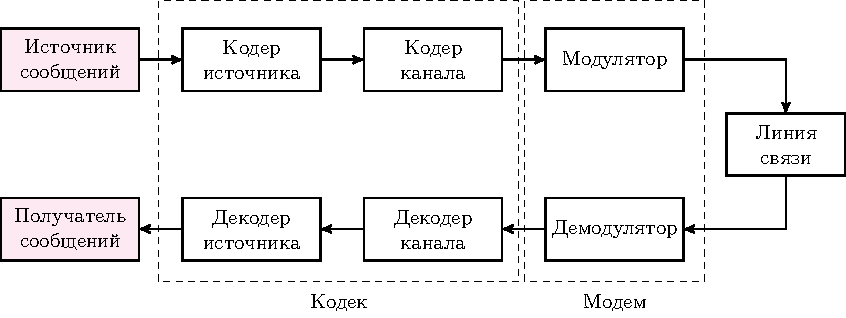
\includegraphics[scale=1]{plot/struct}
	\caption{Структурная схема системы передачи дискретных сообщений}
	\label{fig:2}
\end{figure} 

В частотном модеме используется сигнал с частотной модуляцией. Мы рассмотрим также фазовую модуляцию и спектры модулированных сигналов, а также способ получения частотной модуляции с помощью $RC$-генератора звукового диапазона за счет управления сопротивления канала сток--исток полевого транзистора модулирующим сигналом. 

В эксперименте мы изучим влияние изменения амплитуды или частоты модулирующего колебания на спектр частотно-модулированного (выходного сигнала модулятора) сигнала. 

\section{Краткая теория работы}
\subsection{Сигналы с угловой модуляцией}
В качестве колебания-переносчика используется гармоническое колебание высокой частоты. В процессе модуляции в несущем колебании $f(t)=U_{0} \cos (\omega t+\varphi)$ можно изменять амплитуду (амплитудная модуляция), а также либо частоту $\omega$ (частотная модуляция) либо фазу $\phi$ (фазовая модуляция), оставляя амплитуду постоянной. Поскольку аргумент $\psi=\omega t+\phi$ является полной фазой и определяет текущее значение фазового угла, такие сигналы получили название сигналов с угловой модуляцией.

\subsubsection{Фазовая модуляция (ФМ)}

Если полная фаза процесса $\Psi(t)=\omega_{0} t+k X(t)$, где $X(t)$ - сообщение, $k$ -
коэффициент	пропорциональности,	$\omega_0$ --
значение частоты в отсутствии сообщения $X(t)$, то имеем сигнал с фазовой модуляцией
\begin{equation}
	V_\text{фм}(t)=U_{0} \cos \left[\omega_{0} t+k X(t)\right]
\end{equation}
	
% \begin{figure}[H]

% \end{figure}

\begin{wrapfigure}[19]{r}{0.5\linewidth} 
	\vspace{-2ex}
	\centering
	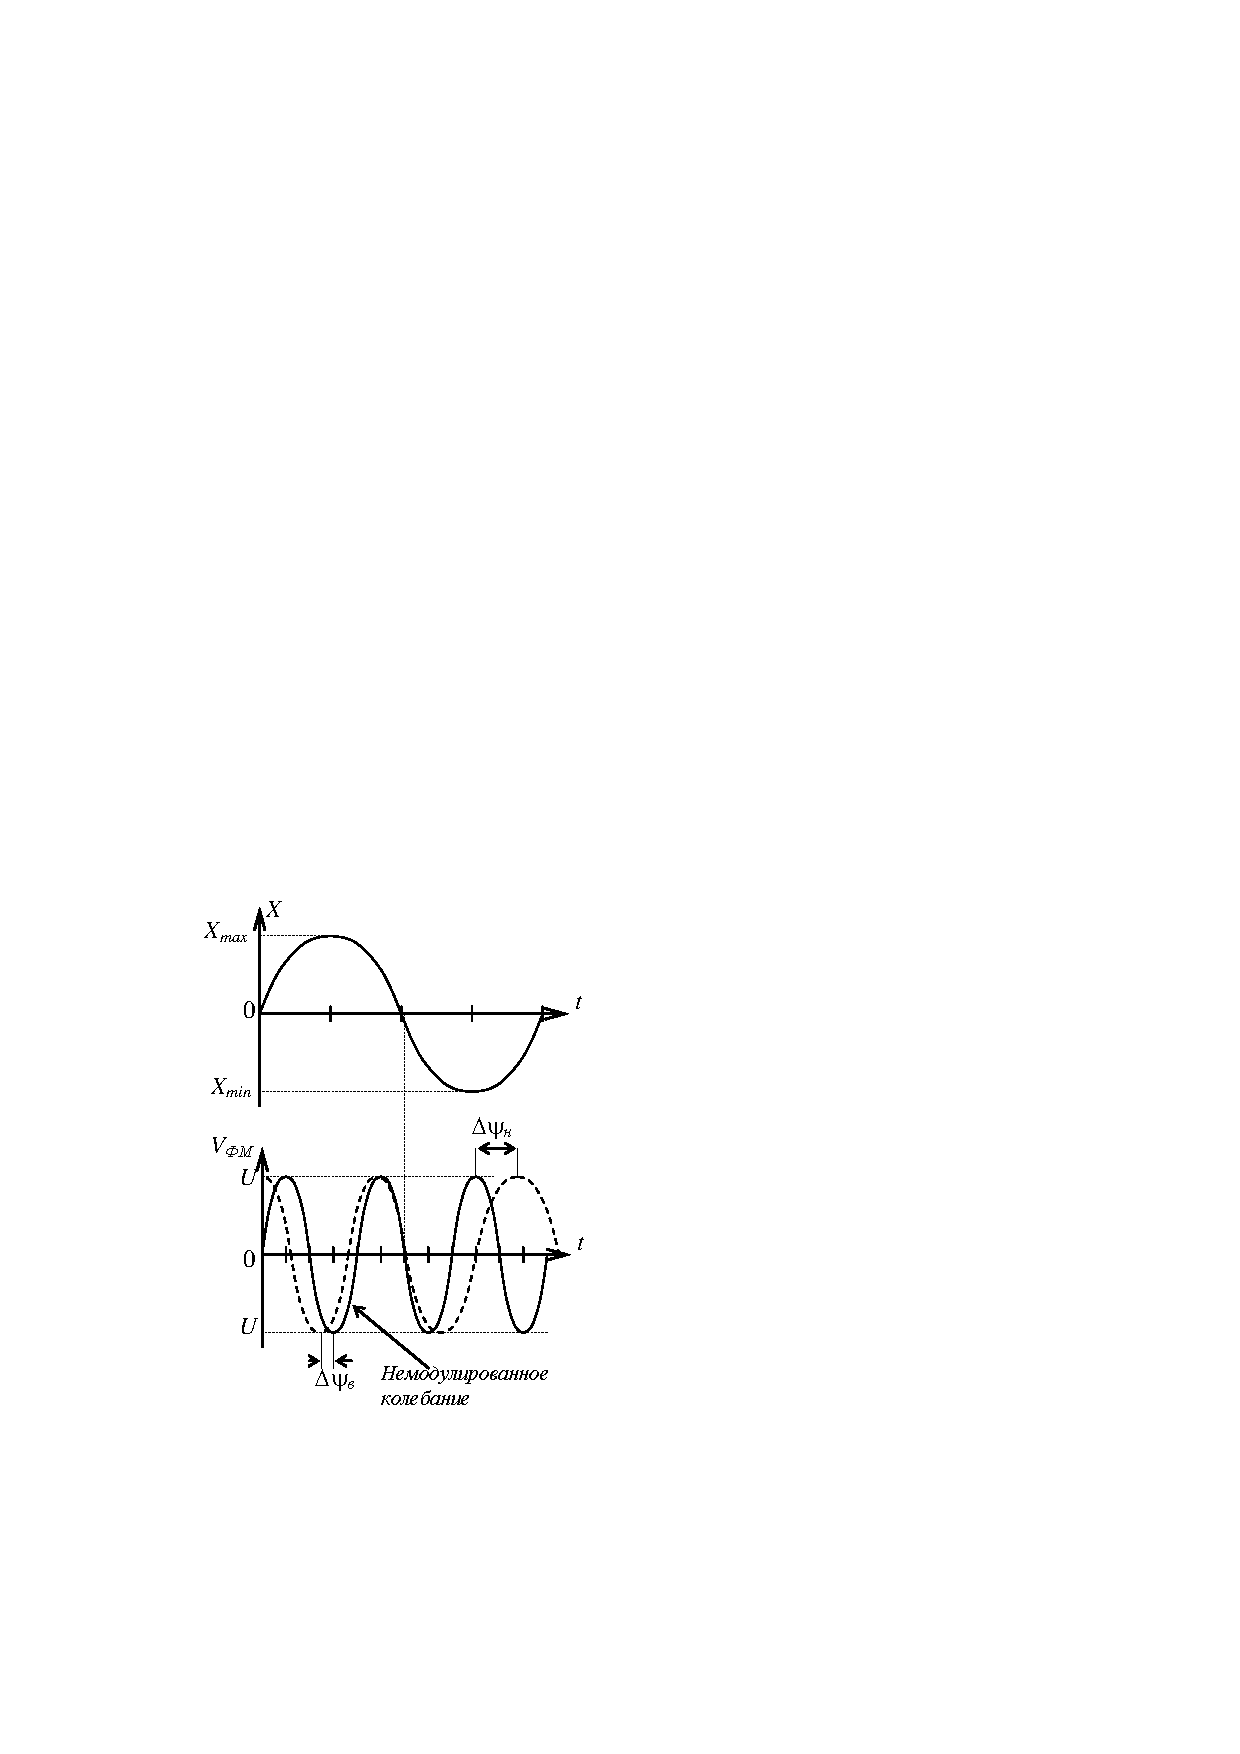
\includegraphics[]{fig/fig2-1}
	\vspace{-1em}
	\caption{}
	\label{fig:2.1}
\end{wrapfigure}

Если сообщение $X(t)=const$, то ФМ-сигнал является простым высокочастотным сигналом.
Если $X(t)=A\cos\Omega t$, то с увеличением значений сообщения $X(t)$ полная фаза $y(t)$ растет во времени быстрее, чем по линейному закону. При уменьшении значений модулирующего сообщения происходит спад скорости роста $y(t)$ во времени (см. рис. \ref{fig:2.1}).



Предельное значение этого фазового сдвига называют девиацией фазы $\Delta \psi$. В общем случае, когда сообщение $X(t)$ изменяет знак, принято различать девиацию фазы вверх $\Delta \psi_v =kX_{max}$ и девиацию фазы вниз $\Delta \psi_n =kX_{min}$.

\subsubsection{Частотная модуляция (ЧМ)}
Мгновенная частота $\omega(t)$ сигнала с угловой модуляцией определяется как первая производная от полной фазы по времени, т.е. мгновенная частота - это скорость изменения полной фазы:
\begin{gather}
	\omega (t)=\dv{\psi}{t}
\end{gather}
Откуда, полная фаза равна:
\begin{equation}
	\label{eq2.1}
	%
	\psi(t)=\int\limits_{0}^{t} \omega(\tau) d \tau+\varphi_{0}
\end{equation}

где $\phi_0$ - начальная фаза в момент времени t=0.
При ЧМ - сигнале между сообщением $X(t)$ и мгновенной частотой $a(t)$ будет связь
вида
\begin{equation}
	\label{eq2.2}
	%
	\omega(t)=\omega_{0}+k X(t)
\end{equation}
Поэтому из \eqref{eq2.1} и \eqref{eq2.2}
\begin{equation}
	%\label{eq2.1}
	V_\text{чм}(t)=U_{0} \cos \psi(t)=U_{0} \cos \left[\int\limits_{0}^{t} \omega(\tau) d \tau+\varphi_{0}\right]
\end{equation}


\begin{equation}
	V_\text{чм}(t)=U_{0} \cos \left[\omega_{0} t+k \int\limits_{0}^{t} X(\tau) d \tau+\varphi_{0}\right]
\end{equation}


\begin{wrapfigure}[11]{l}{0.5\linewidth} 
	\vspace{-2ex}
	\centering
	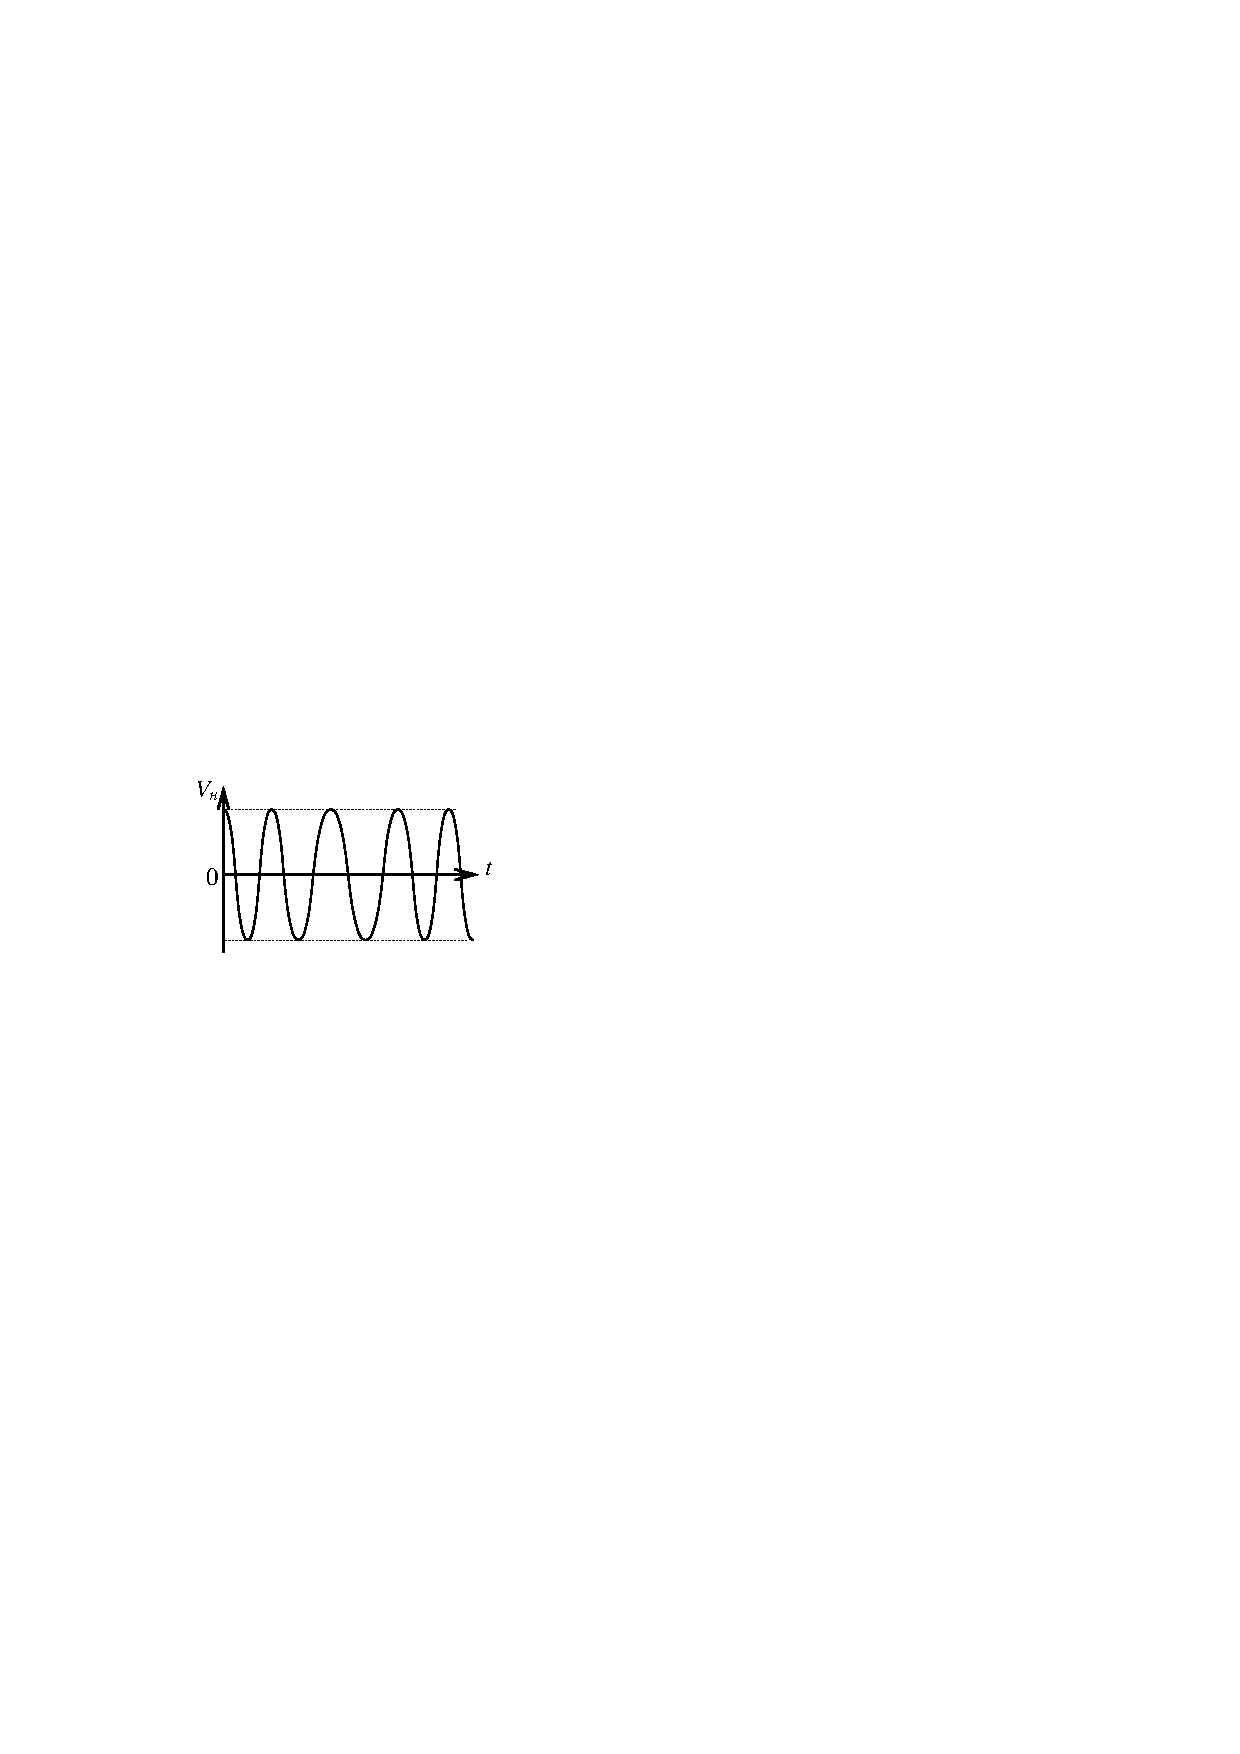
\includegraphics[scale=1.1]{fig/fig2-2}
	\caption{}
	\label{fig:2.2}
\end{wrapfigure}
Если X(t) - достаточно гладкая функция, то внешне осциллограммы ФМ и ЧМ - сигналов не отличаются (рис.2.2). Однако имеет место принципиальная разница: фазовый сдвиг между ФМ - сигналом и с немодулированным пропорционален X(t), для ЧМ этот сдвиг пропорционален интегралу от $X(t)$. Т.е. ЧМ и ФМ - сигналы ведут себя по-разному при изменении частоты модуляции и амплитуды модулирующего колебания.

При ЧМ девиация частоты пропорциональна амплитуде НЧ - сигнала, в то же время девиация частоты $\Delta \omega$ не зависит от частоты $\Omega$ модулирующего сигнала.
\begin{figure}[H]
	\centering
	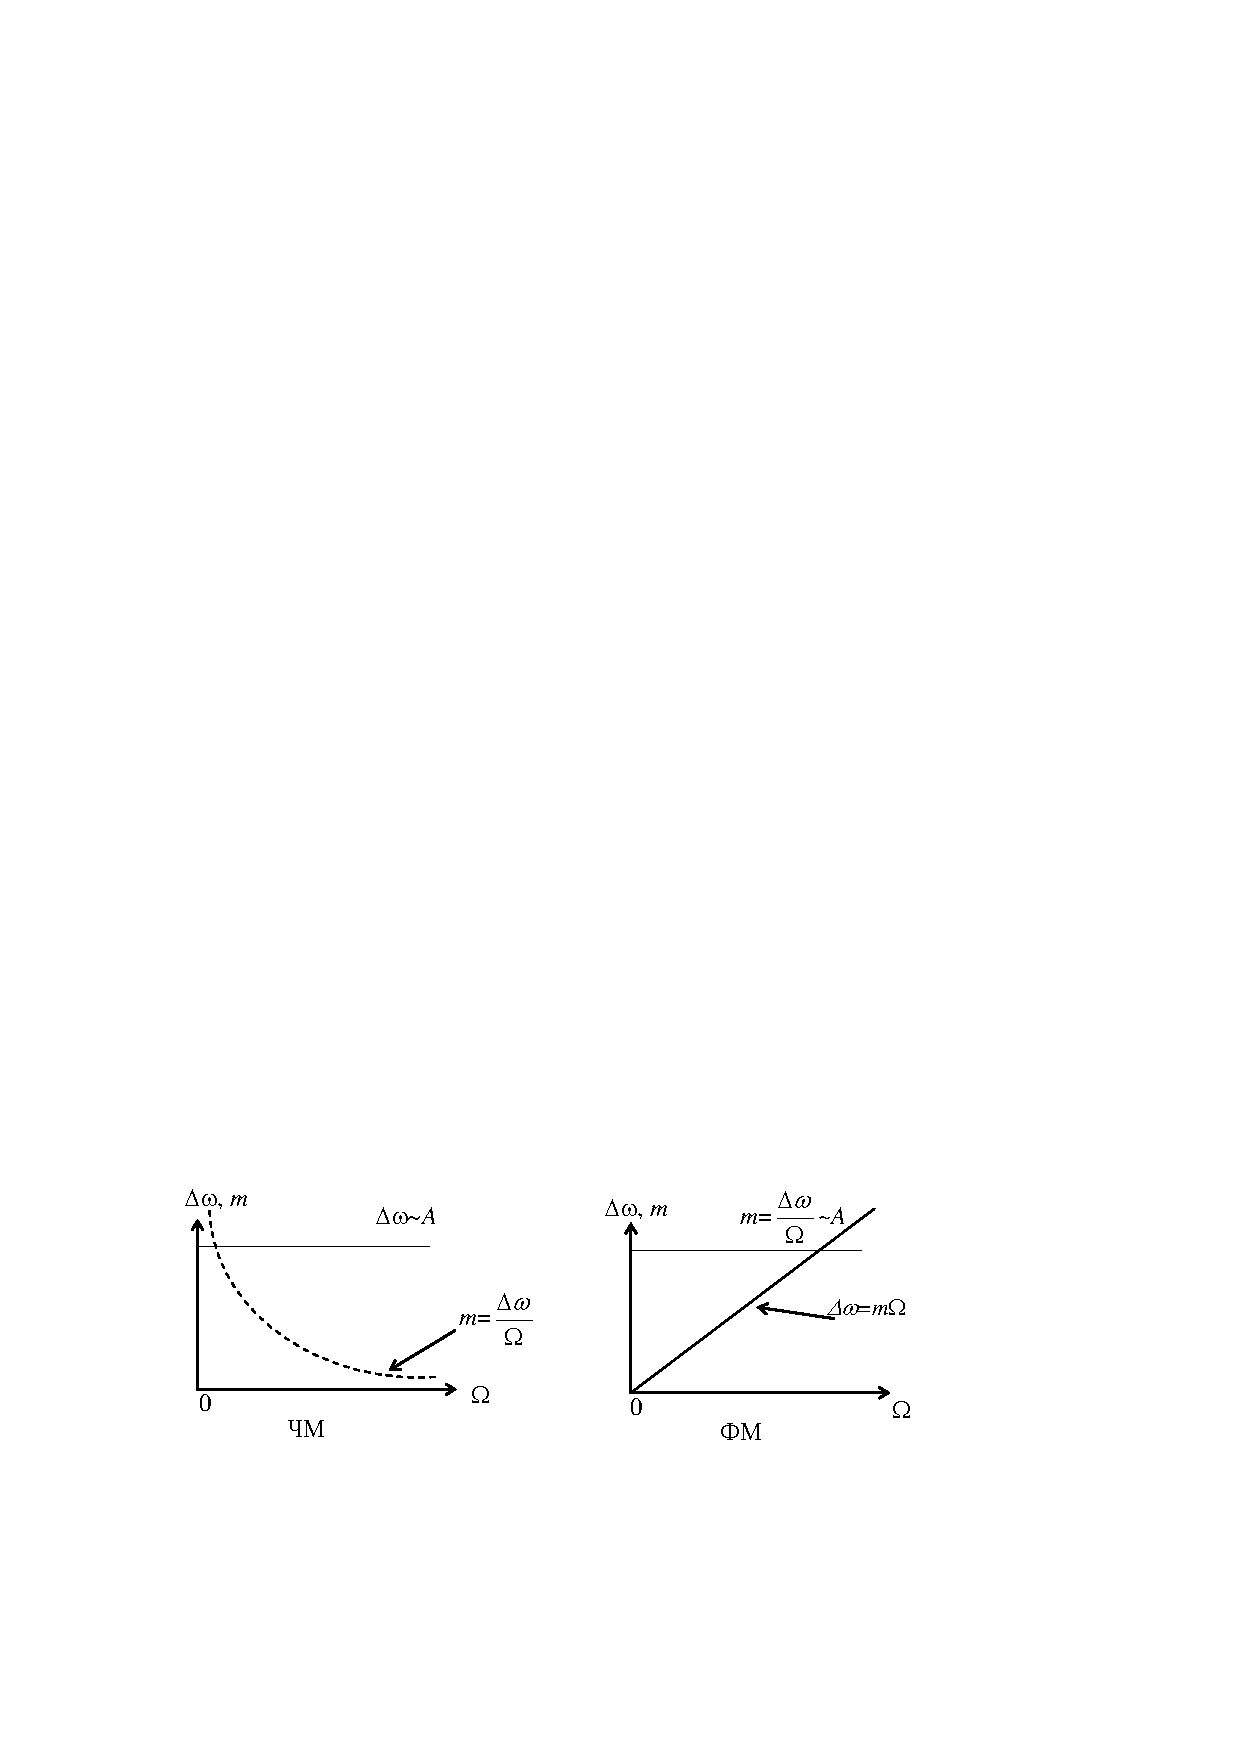
\includegraphics[]{fig/fig2-3}
	\caption{}
	\label{fig:2.3}
\end{figure}
При ФМ индекс модуляции $m=\frac{\Delta \omega}{\Omega} \sim A$ - амплитуде НЧ - сигнала независимо от
частоты модуляции. Как следствие этого, девиация частоты при фазовой модуляции линейно увеличивается с ростом частоты модулирующего сигнала (рис. \ref{fig:2.3}).

\subsubsection{Общие соображения о спектре сигналов с угловой модуляцией}
Если колебание $V(t)=U_{0} \cos [\omega t+\varphi(t)]$
получено с помощью ФМ, то $\phi(t)$ и X(t) полностью совпадают по форме и отличаются лишь постоянными коэффициентами. При этом , с точностью до постоянного коэффициента совпадают спектры функций $\phi(t)$ и X(t).
При ЧМ функция $\phi(t)$ является интегралом от передаваемого сообщения X(t). При ЧМ спектр функции $\phi(t)$ состоит из тех же компонент, что и спектр сообщения X(t), но с измененными амплитудами и фазами.

 Модулированное по углу колебание можно рассматривать как сумму двух квадратурных колебаний: косинусного uc и синусного us, каждое из которых модулировано только по амплитуде. 
\begin{equation}
\label{eq3.3}
	%
	V(t)=U_{0} \cos \varphi(t) \cos \omega_{0} t-U_{0} \sin \varphi(t) \sin \omega_{0} t=u_{c}(t)-u_{s}(t)
\end{equation}
 Закон AM для косинусного колебания определяется медленной функцией $\cos(t)$, для синусного - функцией $\sin(t)$. Но для определения спектра AM колебания достаточно сдвинуть на частоту оо спектр огибающей амплитуд. Следовательно, для нахождения спектра колебания $u(t)$, определяемого выражением \eqref{eq3.3}, необходимо найти сначала спектры функций $\cos(t)$ $\sin(t)$, т.е. спектры огибающих квадратурных колебаний.

Из приведенных рассуждений следует, что при одном и том же передаваемом сообщении спектр колебания, модулированного по углу, значительно сложнее, чем спектр модулированного по амплитуде. Действительно, т.к. $\cos(t)$ и $\sin(t)$ являются нелинейными функциями своего аргумента $\phi(t)$, то спектры этих колебаний могут существенно отличаться от спектра функции $\phi(t)$.


\subsubsection{Спектр ЧМ и ФМ при малых индексах модуляции} % (fold)
	
Задачу о представлении сигналов с угловой модуляцией посредством суммы гармонических колебаний несложно решить в том случае, когда $m\ll 1$. Для тонально-модулированного колебания $V(t)=U_{0} \cos \left[\omega_{0} t+m\sin \Omega t\right]$

\begin{equation}
	V(t)=U_{0} \cos (m \sin \Omega) \cos \omega_{0} t-U_{0} \sin (m \sin \Omega t) \sin \omega_{0} t_{0}
\end{equation}

при $m\ll 1$ $\cos (m \sin \Omega t) \approx 1$, $\sin (m \sin \Omega t) \approx m \sin \Omega t$

\begin{equation}
	V(t) \approx U_{0} \cos \omega_{0} t-U_{0} m \sin \Omega t \cdot \sin \omega_{0} t
\end{equation}

\begin{figure}[h!]
	% \vspace{-2ex}
	\centering
	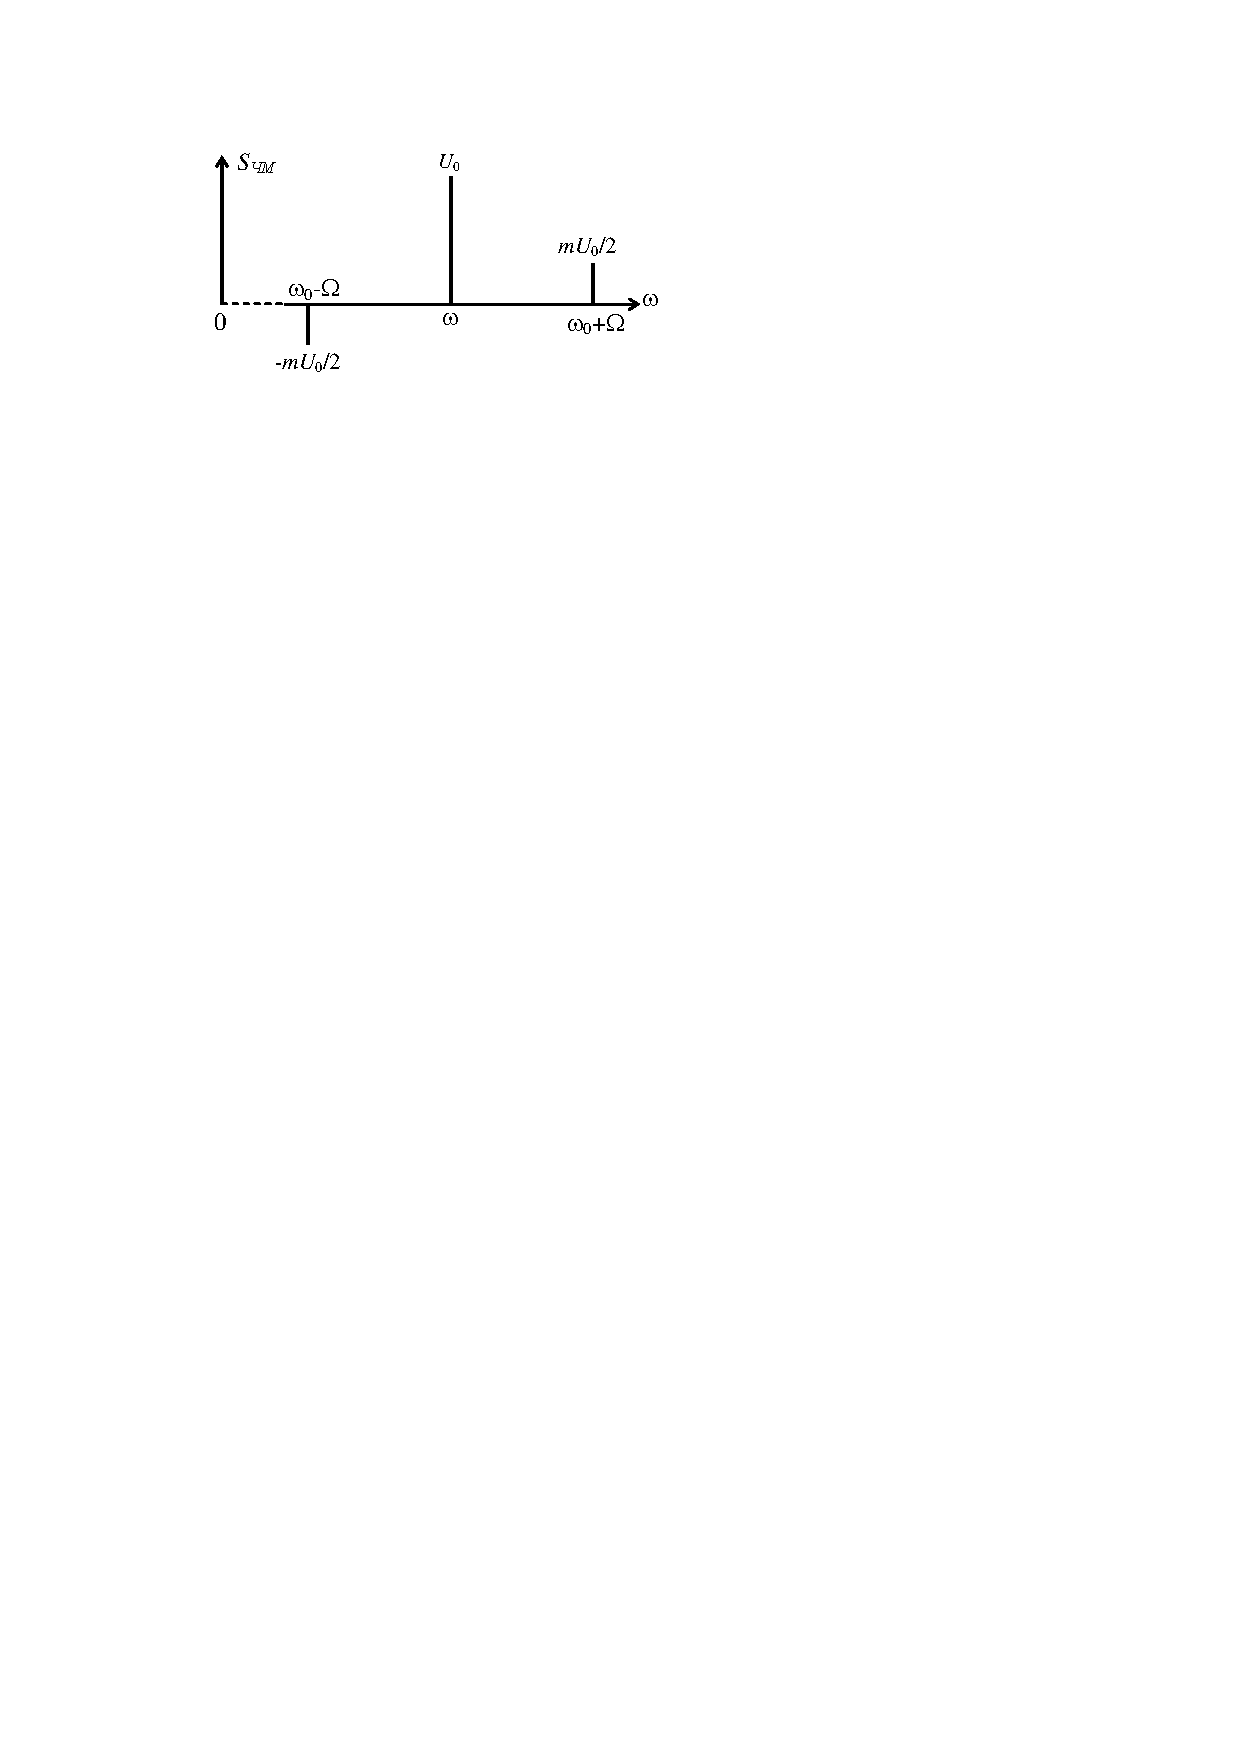
\includegraphics[]{fig/fig2-4}
	\caption{}
	\label{fig:2.4}
	% \label{fig:figure1}
\end{figure}

\begin{equation}
	V(t) \approx U_{0} \cos \omega_{0} t+\frac{m U_{0}}{2} \cos \left(\omega_{0}+\Omega\right) t-\frac{m U_{0}}{2} \cos \left(\omega_{0}-\Omega\right) t
\end{equation}


Таким образом, при $m\ll 1$ в спектре сигнала с угловой модуляцией содержатся несущая и верхняя и нижняя боковые компоненты. Индекс m играет здесь такую же роль, как и в AM - сигнале.
Однако колебание нижних боковых частот имеет сдвиг по фазе 180°.

\subsubsection{Спектр сигнала с угловой модуляцией при произвольном значении индекса модуляции}
Итак, при тональной угловой модуляции
\begin{equation}
	U(t)=U_{0} \cos \left(\omega_{0} t+m \sin \Omega t\right)=U_{0} \operatorname{Re}\left(e^{j \omega_{0} t} \cdot e^{j m \sin \Omega t}\right)
\end{equation}
\begin{equation}
	e^{j m \sin Z}=\sum_{k=-\infty}^{\infty} J_{k}(m) e^{j k Z}
\end{equation}
где $m$ - любое вещественное число, $J_{k}(m)$ - функция Бесселя k порядка от аргумента $m$. 
Представляя экспоненту в виде ряда, получим модель ЧМ-ФМ сигнала  с любым значением индекса модуляции:
\begin{equation}
	U(t)=U_{0} \sum_{k=-\infty}^{\infty} J_{k}(m) \cos \left(\omega_{0}+k \Omega\right)
\end{equation}
При $m\ll 1$ ширина спектра ЧМ как и АМ равна $2\Omega$, при значении $m$ от 0.5 до 1 приобретает значение вторая пара боковых частот, поэтому ширина спектра равна $4\Omega$.
\begin{figure}[H]
	\centering
	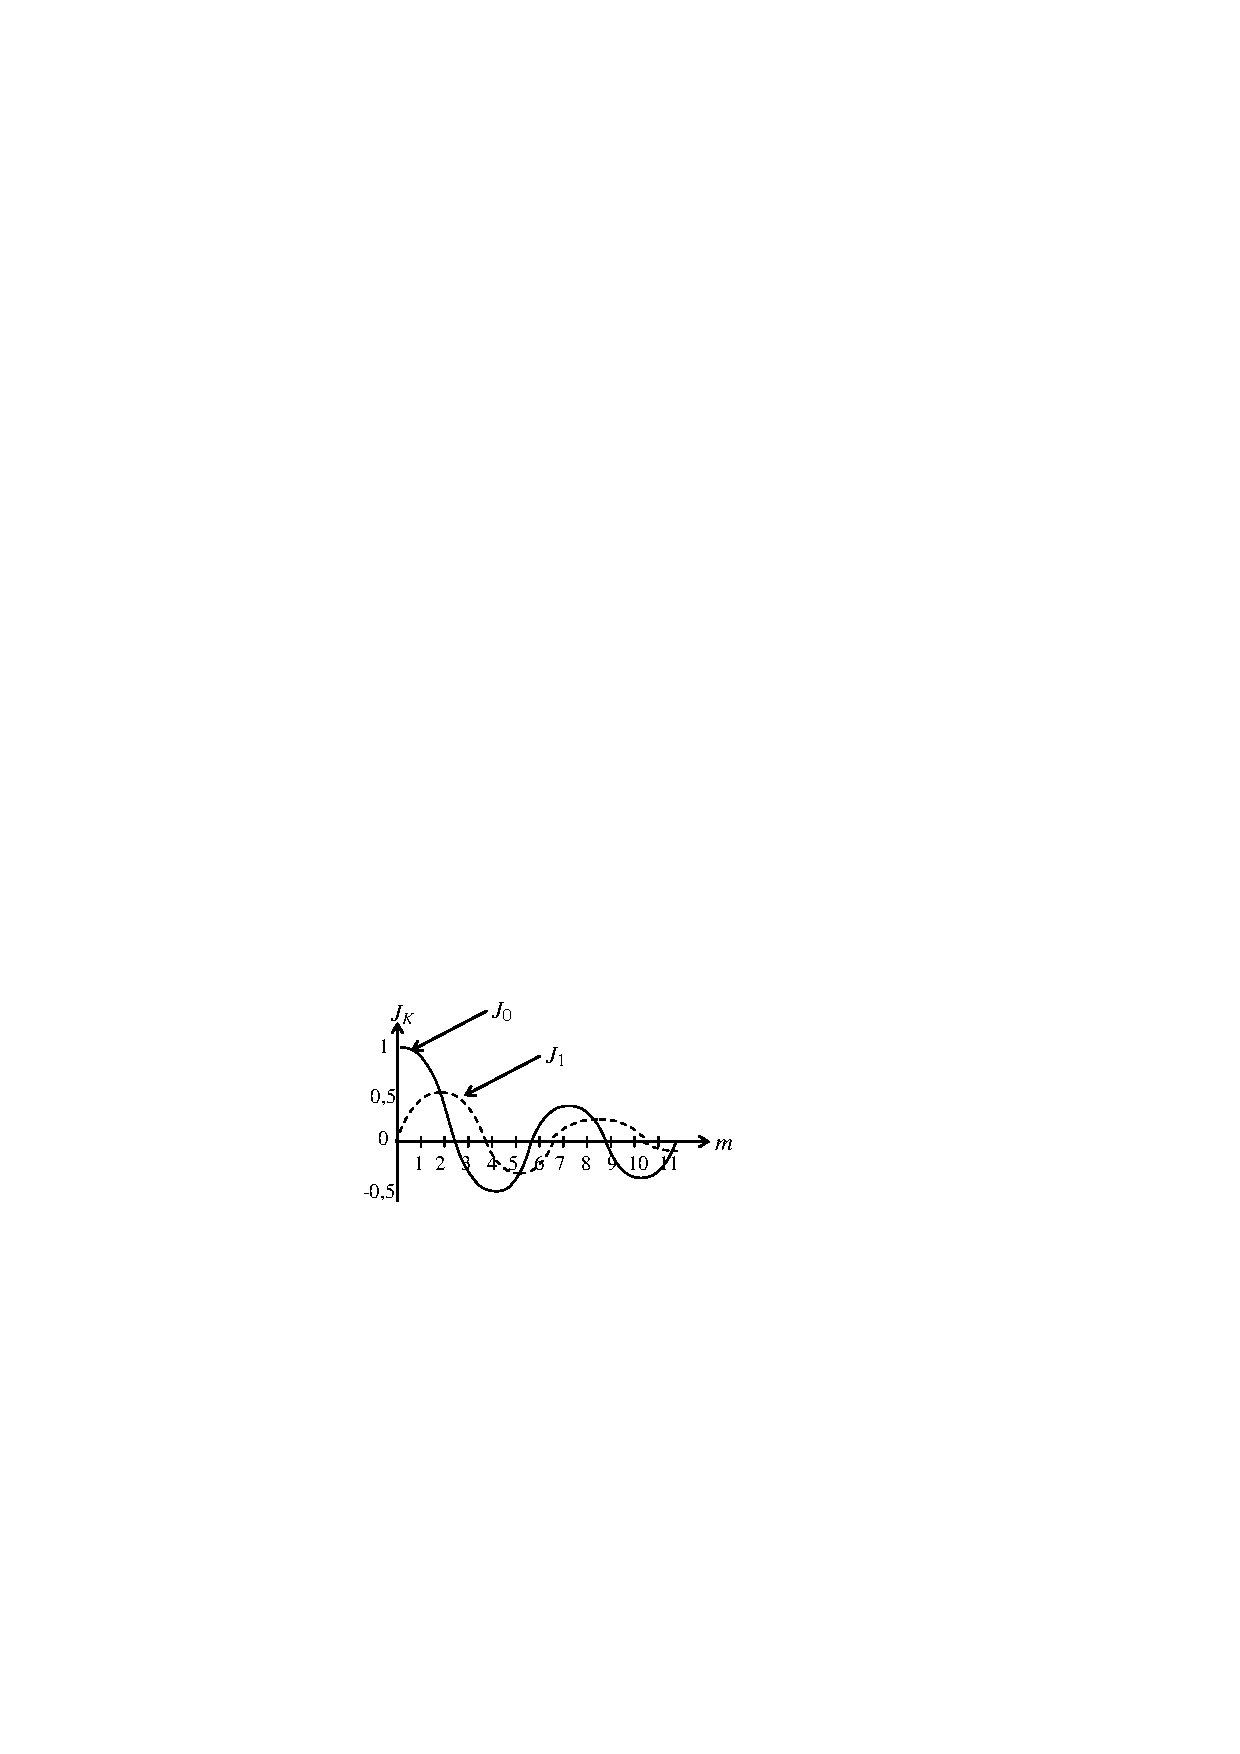
\includegraphics[]{fig/fig2-5}
	\caption{}
	\label{fig:2.5}
	% \label{fig:figure1}
\end{figure}

\begin{figure}[H]
	\centering
	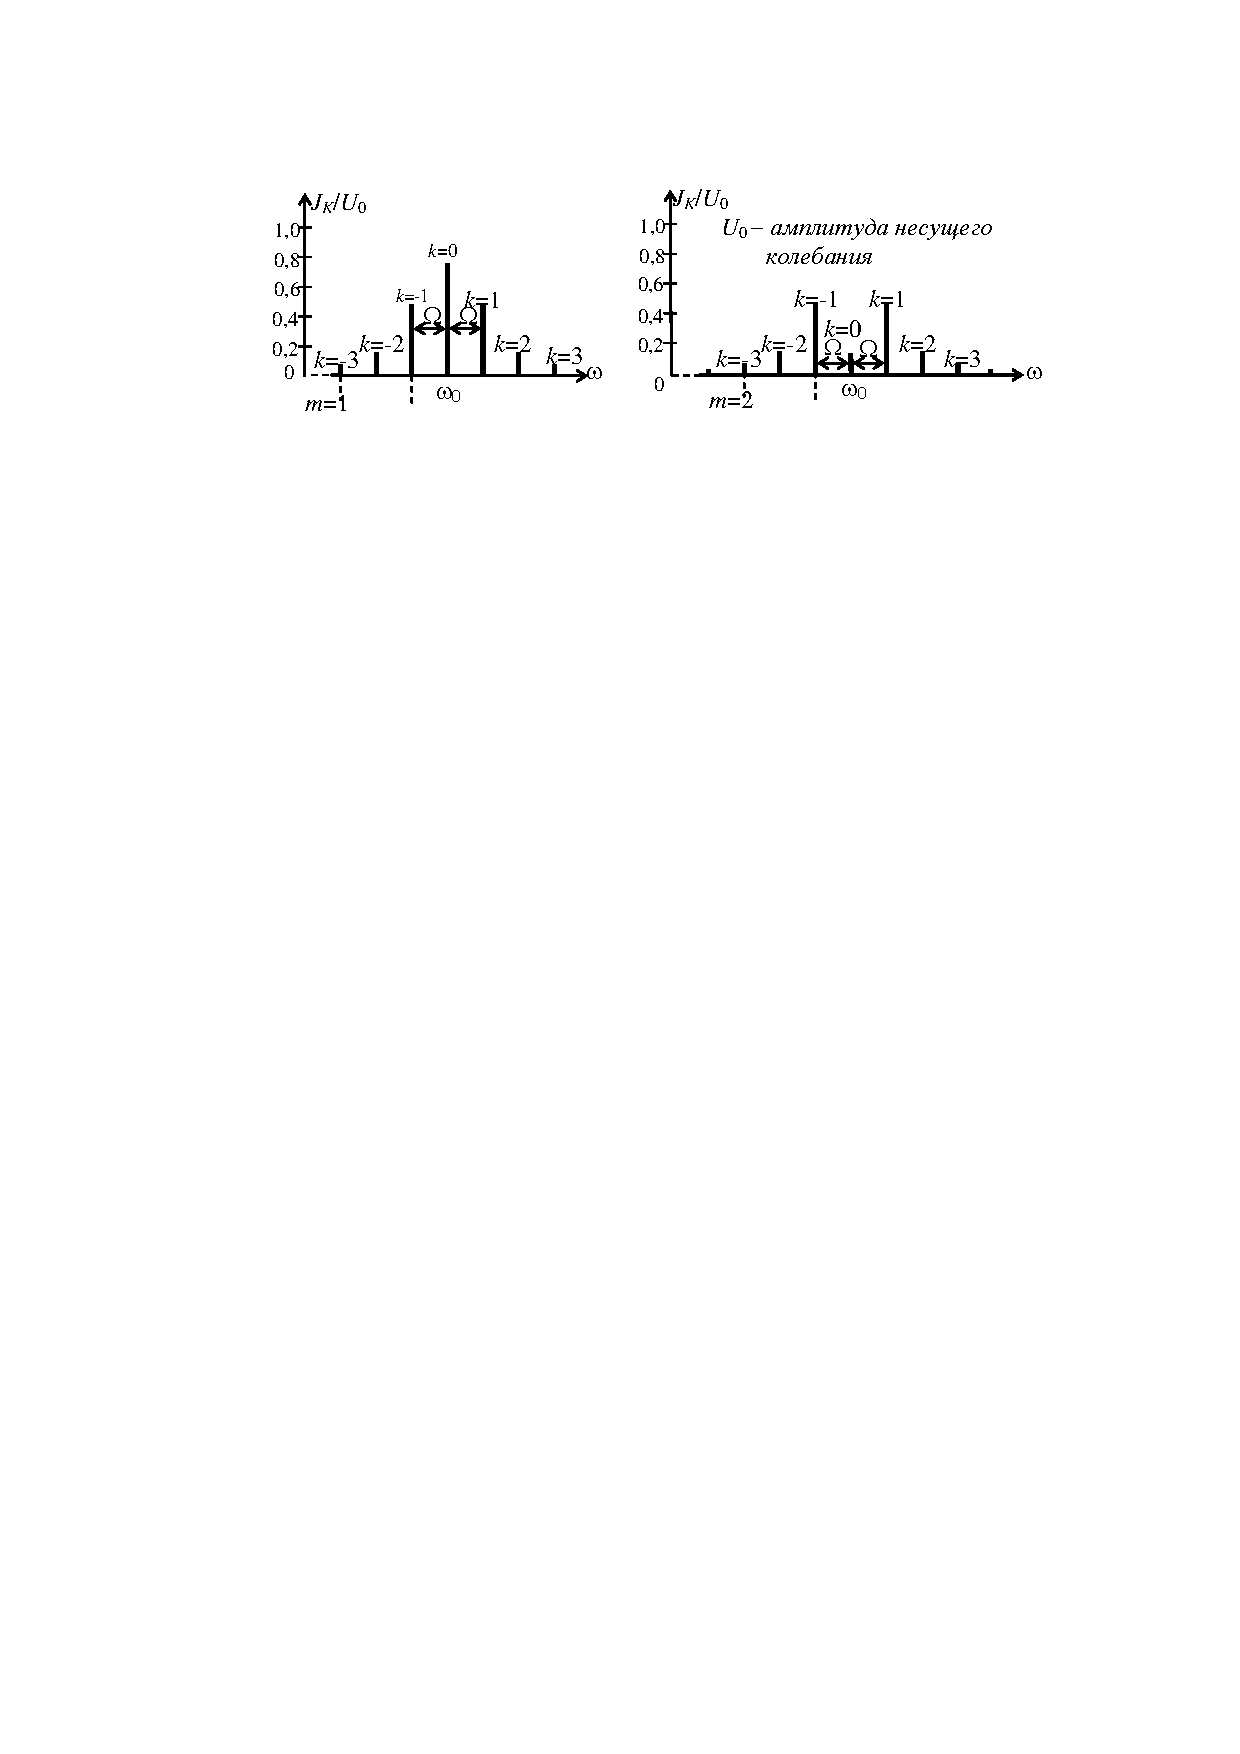
\includegraphics[]{fig/fig2-6}
	\caption{}
	\label{fig:2.6}
	% \label{fig:figure1}
\end{figure}
Фазы колебаний на рисунке \ref{fig:2.6} не учитываются, однако следует иметь в виду что, при нечетных $k$ амплитуды нижних боковых следует брать со знаком минус. 

Чем больше индекс $k$ функции Бесселя, тем протяженнее область аргументов, при которых эта функция мала. Важно отметить, что с ростом индекса модуляции $m$ расширяется полоса частот, занимаемая сигналом. Обычно полагают, что допустимо пренебречь всеми спектральными составляющими с номером $|k|>m+1$. Отсюда следует оценка практической ширины спектра с угловой модуляцией 
\begin{equation}
	\Pi_\text{пр}=2k\Omega=2(m+1)\Omega
	\label{eq:ocenka}
\end{equation}.

Как видно, реальные ЧМ и ФМ - сигналы характеризуются условием $m\gg1$, итак:
\begin{equation}
	\Pi_\text{пр} \approx 2 m \Omega=2 \Delta \omega
\end{equation}

\subsection{Частотная модуляция в автогенераторе}
Задачу получения ЧМ колебаний можно сформулировать как задачу создания генератора гармонических колебаний, частота которого должна изменяться в соответствии с законом изменения управляющего сигнала. Частота колебаний генератора
определяется резонансной частотой контура $\omega_{0}=\frac{1}{\sqrt{L C}}$ и, следовательно, для ее
изменения необходимо менять либо емкость C, либо индуктивность L.
		
Продифференцировав $\omega_0$, например, по C получим $\frac{d \omega_{0}}{d C}=-\frac{\omega_{0}}{2 C}$ или $\frac{\Delta \omega}{\omega_{0}} \approx-\frac{1}{2} \frac{\Delta C}{C_{0}}$.

Как видно, при малых изменениях частоты можно считать, что она пропорциональна емкости, т.е., желая получить модулированное колебание, следует изменить емкость (или индуктивность) контура в соответствии с передаваемым сообщением, поэтому контур должен содержать емкостной (или индуктивный) параметрический элемент.

Широко распространенным способом электронного управления является подключение к контуру варикапа, емкость которого зависит от напряжения, приложенного в направлении запирания перехода.

Упрощенная схема автогенератора с варикапом изображена на рис. \ref{fig:3.2}.
\begin{figure}[H]
	\centering
	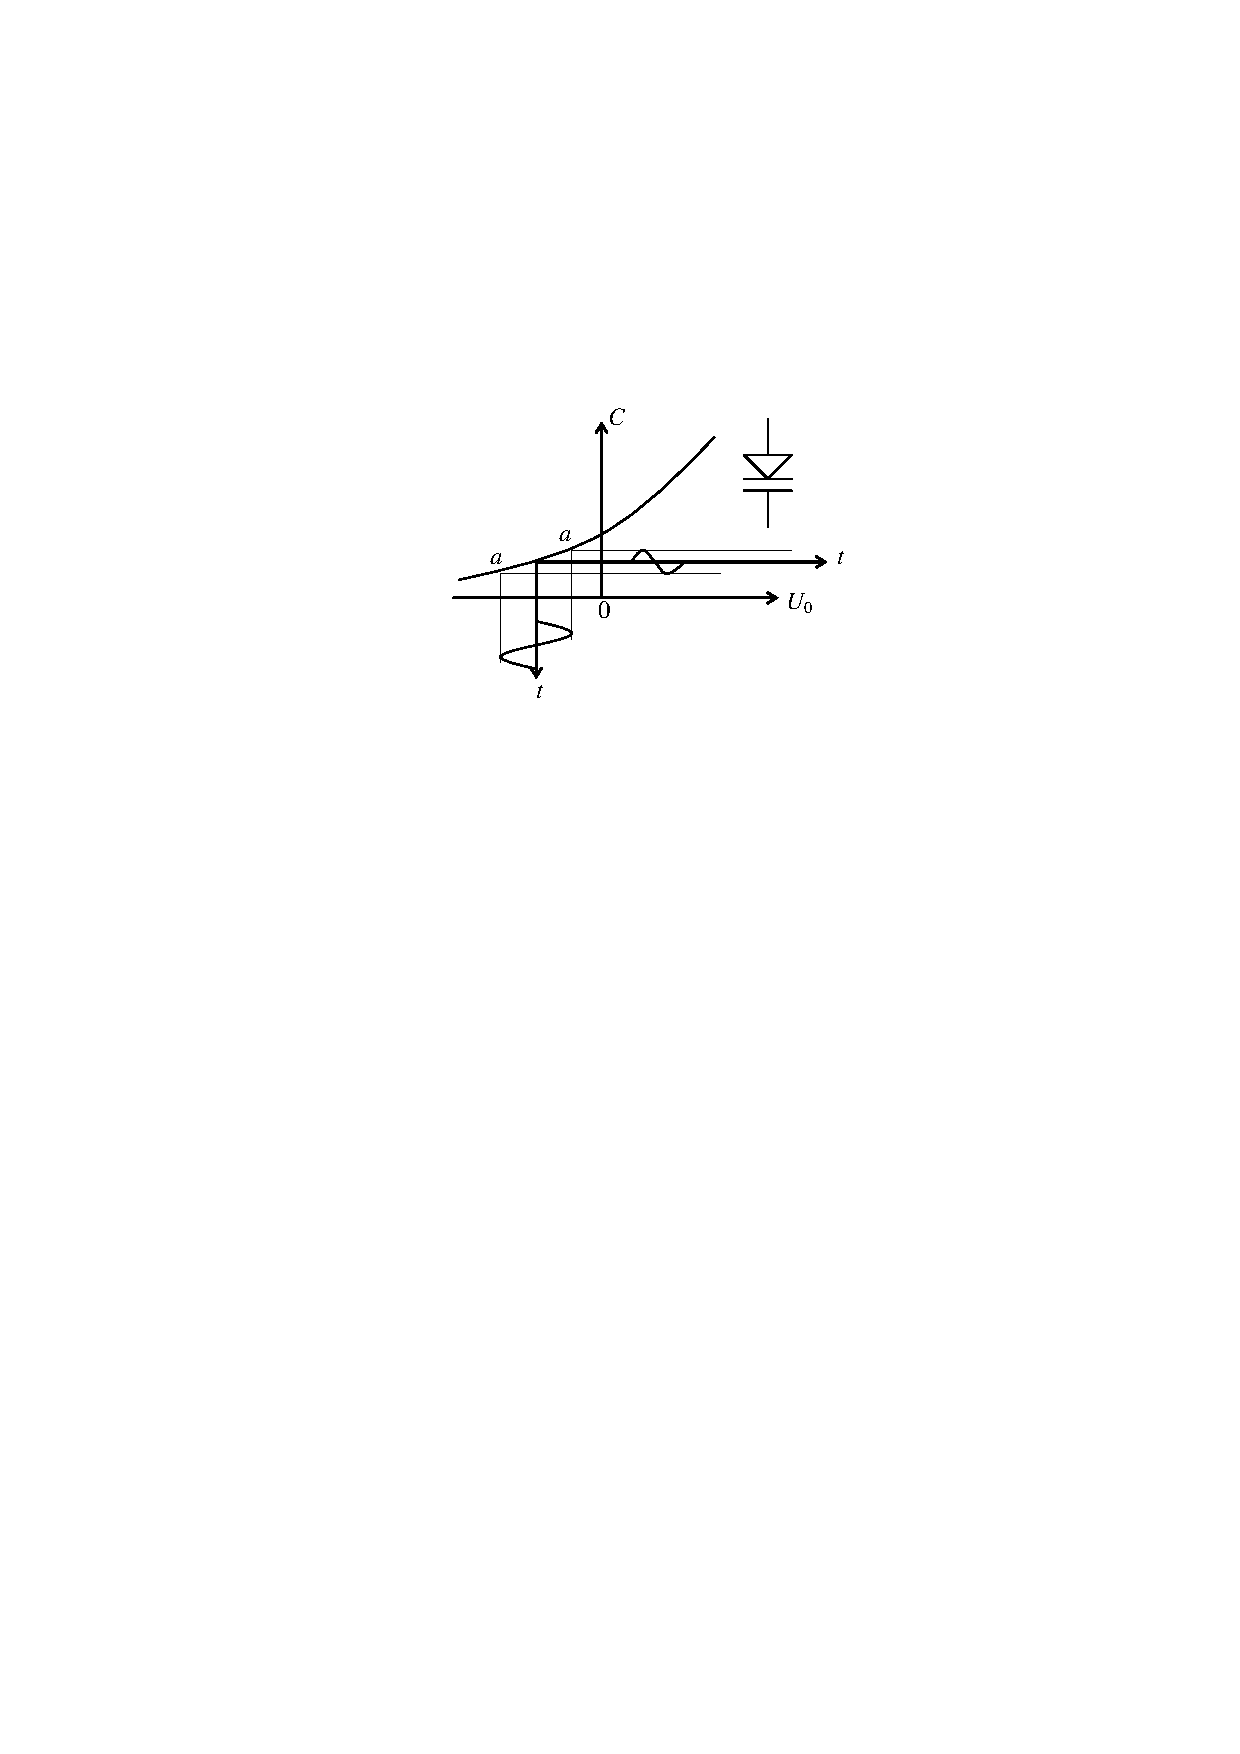
\includegraphics[]{fig/fig3-1}
	\caption{}
	\label{fig:3.1}
	% \label{fig:figure1}
\end{figure}
\begin{figure}[H]
	\centering
	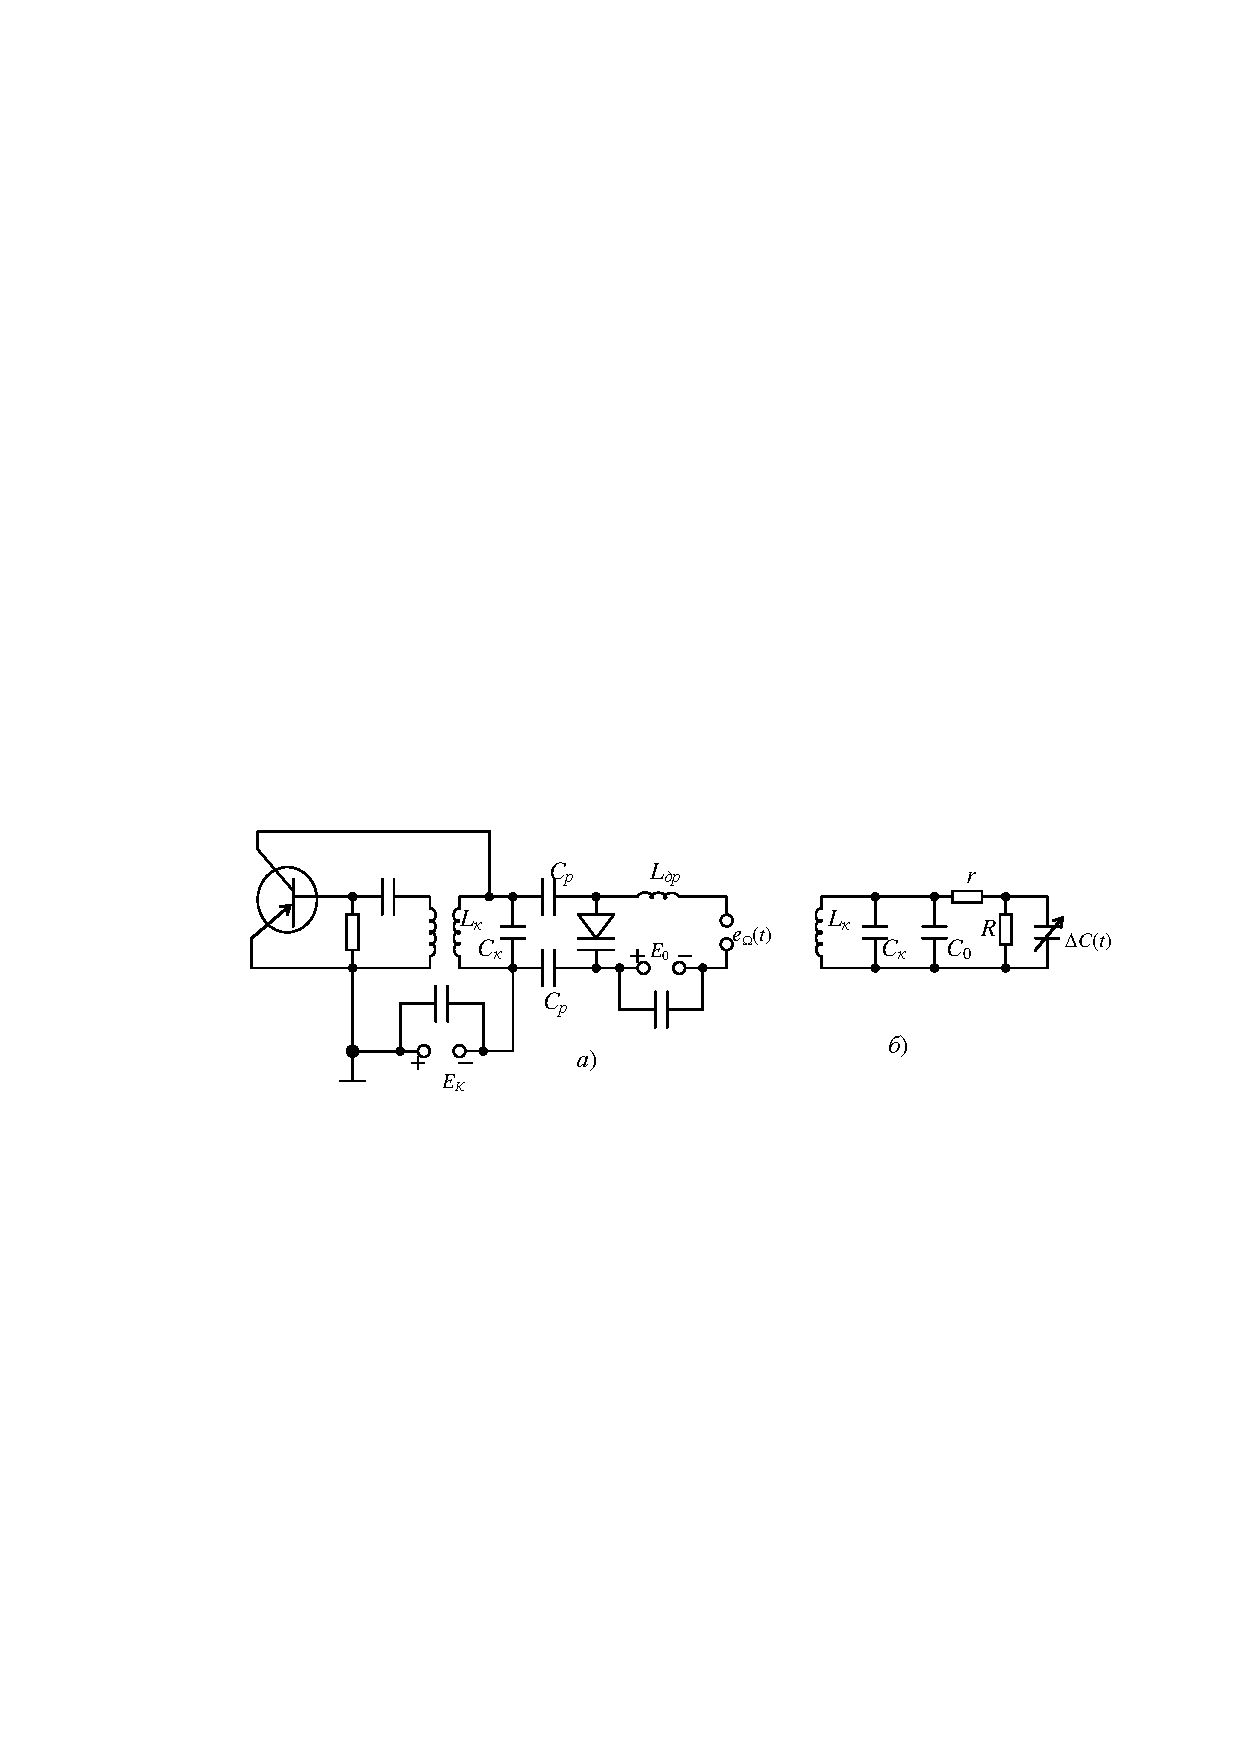
\includegraphics[]{fig/fig3-2}
	\caption{}
	\label{fig:3.2}
	% \label{fig:figure1}
\end{figure}
Разделительный конденсатор $C_p$, предназначен для развязки контура от источника $E_0$. Источник $E_0$ устанавливает начальную рабочую точку (НРТ) на вольт-фарадной характеристике варикапа. Блокировочный дроссель $L_\text{др}$ предназначен для того, чтобы ВЧ ток от автогенератора не проходил в источник ЭДС $e_{\Omega}(t)$.

На схеме замещения (рис. \ref{fig:3.2}б) $C_0$ - средняя емкость в отсутствии модулирующего колебания, $\Delta C(t)$ - вариация емкости в зависимости от  $e_{\Omega}(t)$. Сопротивление p-n перехода R, объемное сопротивление полупроводника г.

Если напряжение на емкости достаточно мало, то, как отмечено выше, нелинейный элемент можно трактовать как линейный параметрический. Принимая рабочий участок <<а-а>> зависимости $C(U)$ (рис. \ref{fig:3.1}) за прямую линию получим следующее.

Если управляющее напряжение меняется по закону $u_{y n p}=E_{0}+U_{c} \cos \Omega t$, то емкость меняется по закону $C=C_{0}\left(1+m_{c} \cos \Omega t\right)$.

\subsection{Демодуляция ЧМ-сигналов}

При частотной модуляции, как известно, полезное сообщение пропорционально отклонению мгновенной частоты сигнала от частоты несущего колебания $\omega(t)-\omega_0$, где $\omega(t)=\omega_{0}+\Delta \omega \cos \Omega t$:
\begin{equation}
	U_\text{чм}(t)=E_{0} \cos \left[\omega_{0}+\Delta \omega \cos \Omega t\right] t
\end{equation}

ЧМ детектирование можно осуществить преобразованием ЧМ-сигнала в неглубокий АМ-сигнал и дальнейшим амплитудным детектированием. 
Для этого нужно подать ЧМ-сигнал на линейный частотный фильтр, настроенный таким образом, чтобы несущая частота ЧМ-сигнала попадала на линейный участок фильтра. АЧХ полосового фильтра можно разложить в ряд:
\begin{equation}
	\label{eq4.1}
	|K(j \omega)|=
	\qty|K(j \omega_{0})|+
	\qty|\dv{K(j\omega_0)}{\omega}|\cdot\qty(\omega(t)-\omega_0)+\ldots
\end{equation}

Тогда на выходе фильтра получится сигнал со сложной амплитудно-угловой модуляцией с мгновенной амплитудой переменной составляющей
\begin{equation}
	V_\text{вых}(t)=b_{0}\cdot\qty|\dv{K(j\omega_0)}{\omega}|\cdot \Delta \omega \cos \Omega t,
\end{equation}
где $b_0$ -- постоянный коэффициент. Окончательная обработка проводится обычным AM детектором, включаемым на выходе фильтра.

Этот метод имеет недостаток, обусловленный малым диапазоном линейности характеристики детектирования и необходимостью настройки на частоту, отличную от частоты немодулированного колебания ($\omega_{\text{рез}} \neq \omega_{0}$).

Для устранения этого недостатка совмещают в одной схеме два контура и два амплитудных детектора таким образом, что контуры настроены на частоты, симметрично смещенные относительно несущей, и при этом выходы двух детекторов соединены так, что их выходные напряжения вычитаются друг из друга. В этом случае детекторная характеристика будет иметь достаточно протяженный, почти линейный участок.

\subsection{$RC$--генератор низкочастотных гармонических колебаний}

В нашей установке был использован $RC$-автогенератор гармонических колебаний звукового диапазона в составе частотного модулятора.

Рассмотрим уравнение автогенератора с $LC$-контуром:
\begin{gather}
	\label{eq5.1}
	\dv[2]{U}{t}+
	\qty(
		\frac{R}{L} - 
		\frac{M}{LC}\dv{\varphi(U)}{U}
	)\dv{U}{t}+
	\omega_r^2U=0
\end{gather}
Это уравнение имеет второй порядок. Действием обратной связи, реализованной на трансформаторной связи с взаимной индуктивностью $М$, коэффициент при первой производной 
$\qty(
	\frac{R}{L} - 
	\frac{M}{LC}\dv{\varphi(U)}{U}
)$  
обращается в нуль в стационарном режиме и отрицательна в режиме самовозбуждения. Для создания $RC$-автогенератора нужно так составить схему, чтобы она описывалась таким же дифференциальным уравнением второго порядка, как и \eqref{eq5.1}. Рассмотрим схему, представленную на рис. \ref{fig:5.1}. 
\begin{figure}[H]
	\centering
	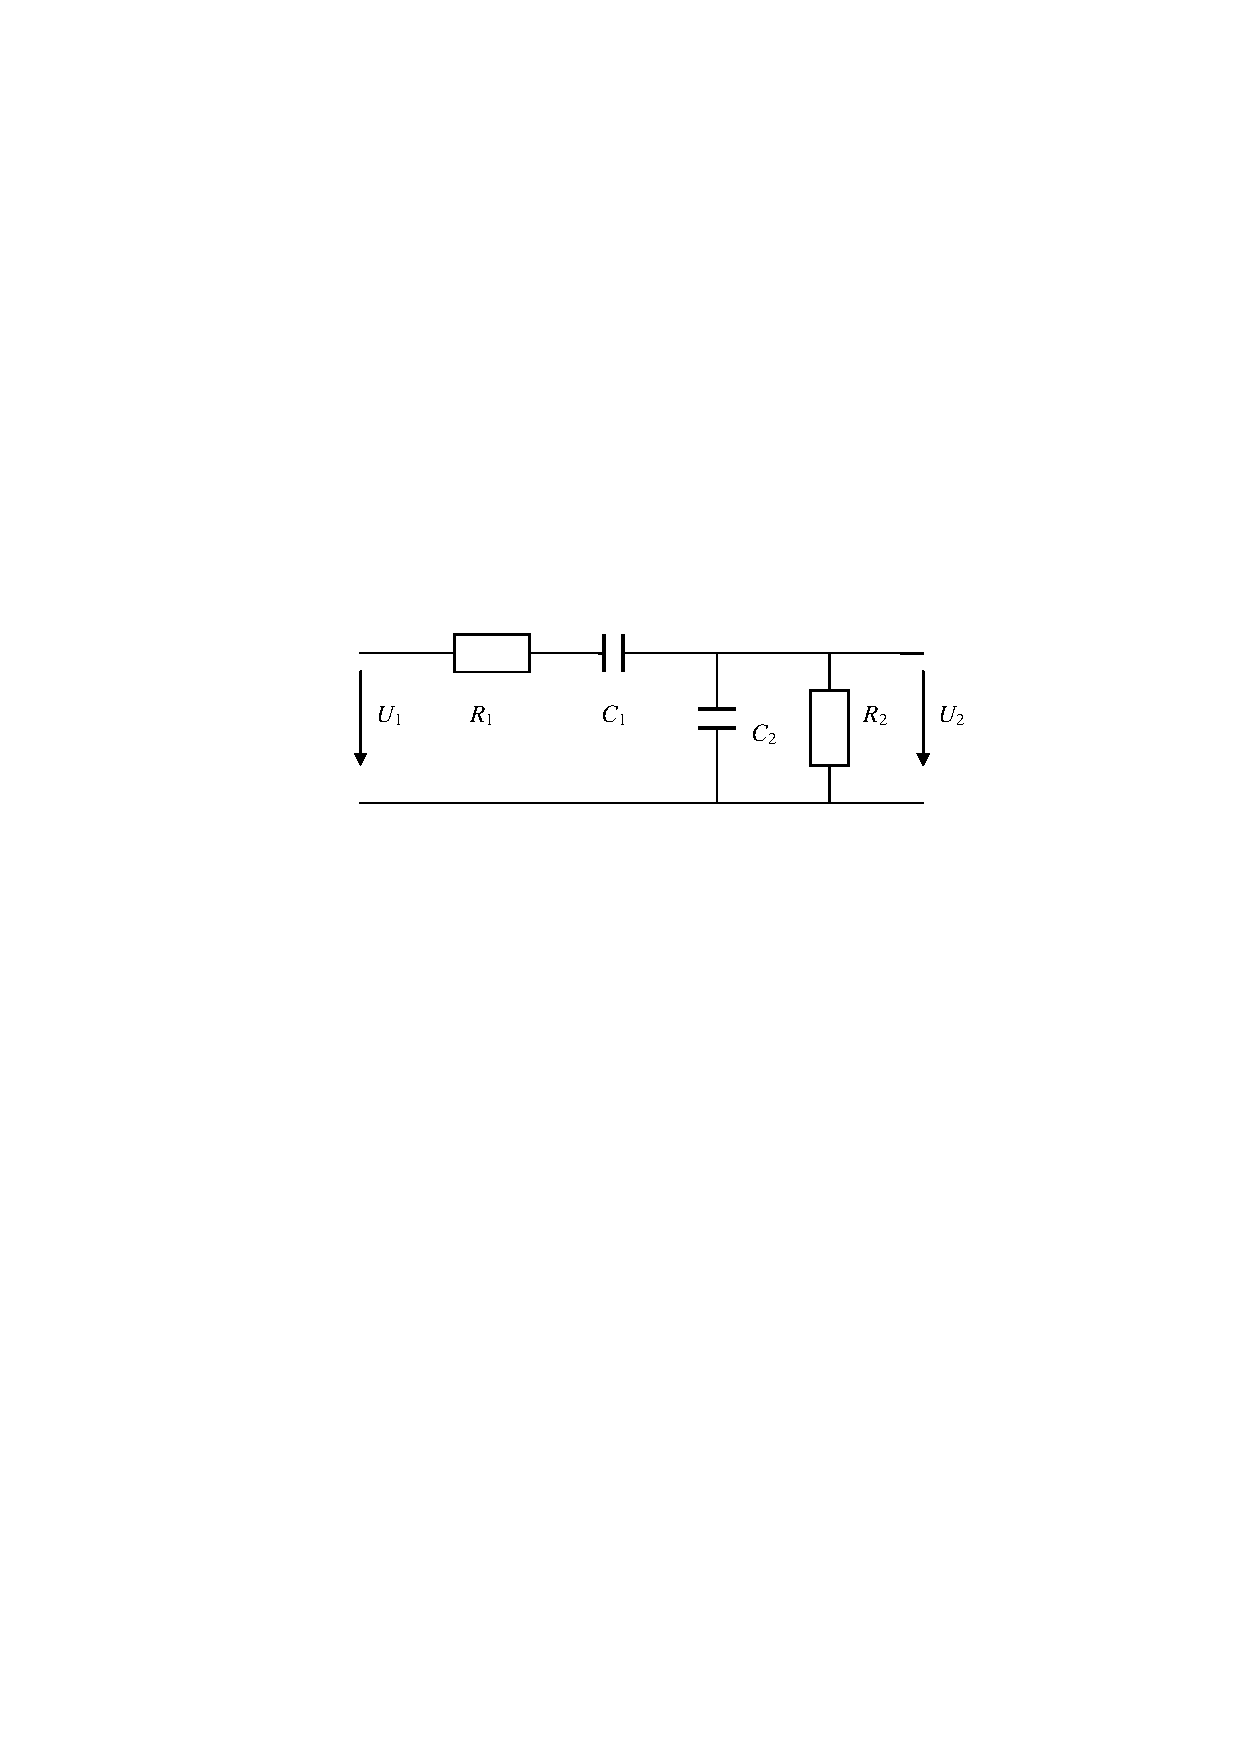
\includegraphics[]{fig/fig5-1.pdf}
	\caption{}
	\label{fig:5.1}
\end{figure}
Дифференциальное уравнение этой схемы
\begin{gather}
	\label{eq5.2}
	%
	\dv{U_2}{t}+
		2 \alpha U_2 + 
		\omega_0^2\int\limits_0^t U_2\, \dd t=
		\frac{U_1}{\tau_{12}}
	\quad \Rightarrow \quad
	%
	\dv[2]{U_2}{t}+
		2 \alpha \dv{U_2}{t} + 
		\omega_0^2 U_2 =
		\frac{1}{\tau_{12}}	\dv{U_1}{t},\\
	%
	\text{где} \quad
	\omega_0^2=\frac{1}{R_1 R_2 C_1 C_2}, \quad
	2 \alpha=\frac{1}{\tau_1}+\frac{1}{\tau_2}+\frac{1}{\tau_{12}}, \quad
	\tau_1=R_1C_1, \quad \tau_2=R_2C_2, \quad \tau_{12}=R_1C_2.
\end{gather}
Левая часть уравнения \eqref{eq5.2} совершенно аналогична левой части уравнения \eqref{eq5.1}. Если теперь в эту схему внести нелинейный усилитель и охватить всю схему обратной связью, как показано на рис.  \ref{fig:5.2}, то полученная схема сможет генерировать гармонические колебания на одной из частот, определяемых уравнением \eqref{eq5.2}.
\begin{figure}[H]
	\centering
	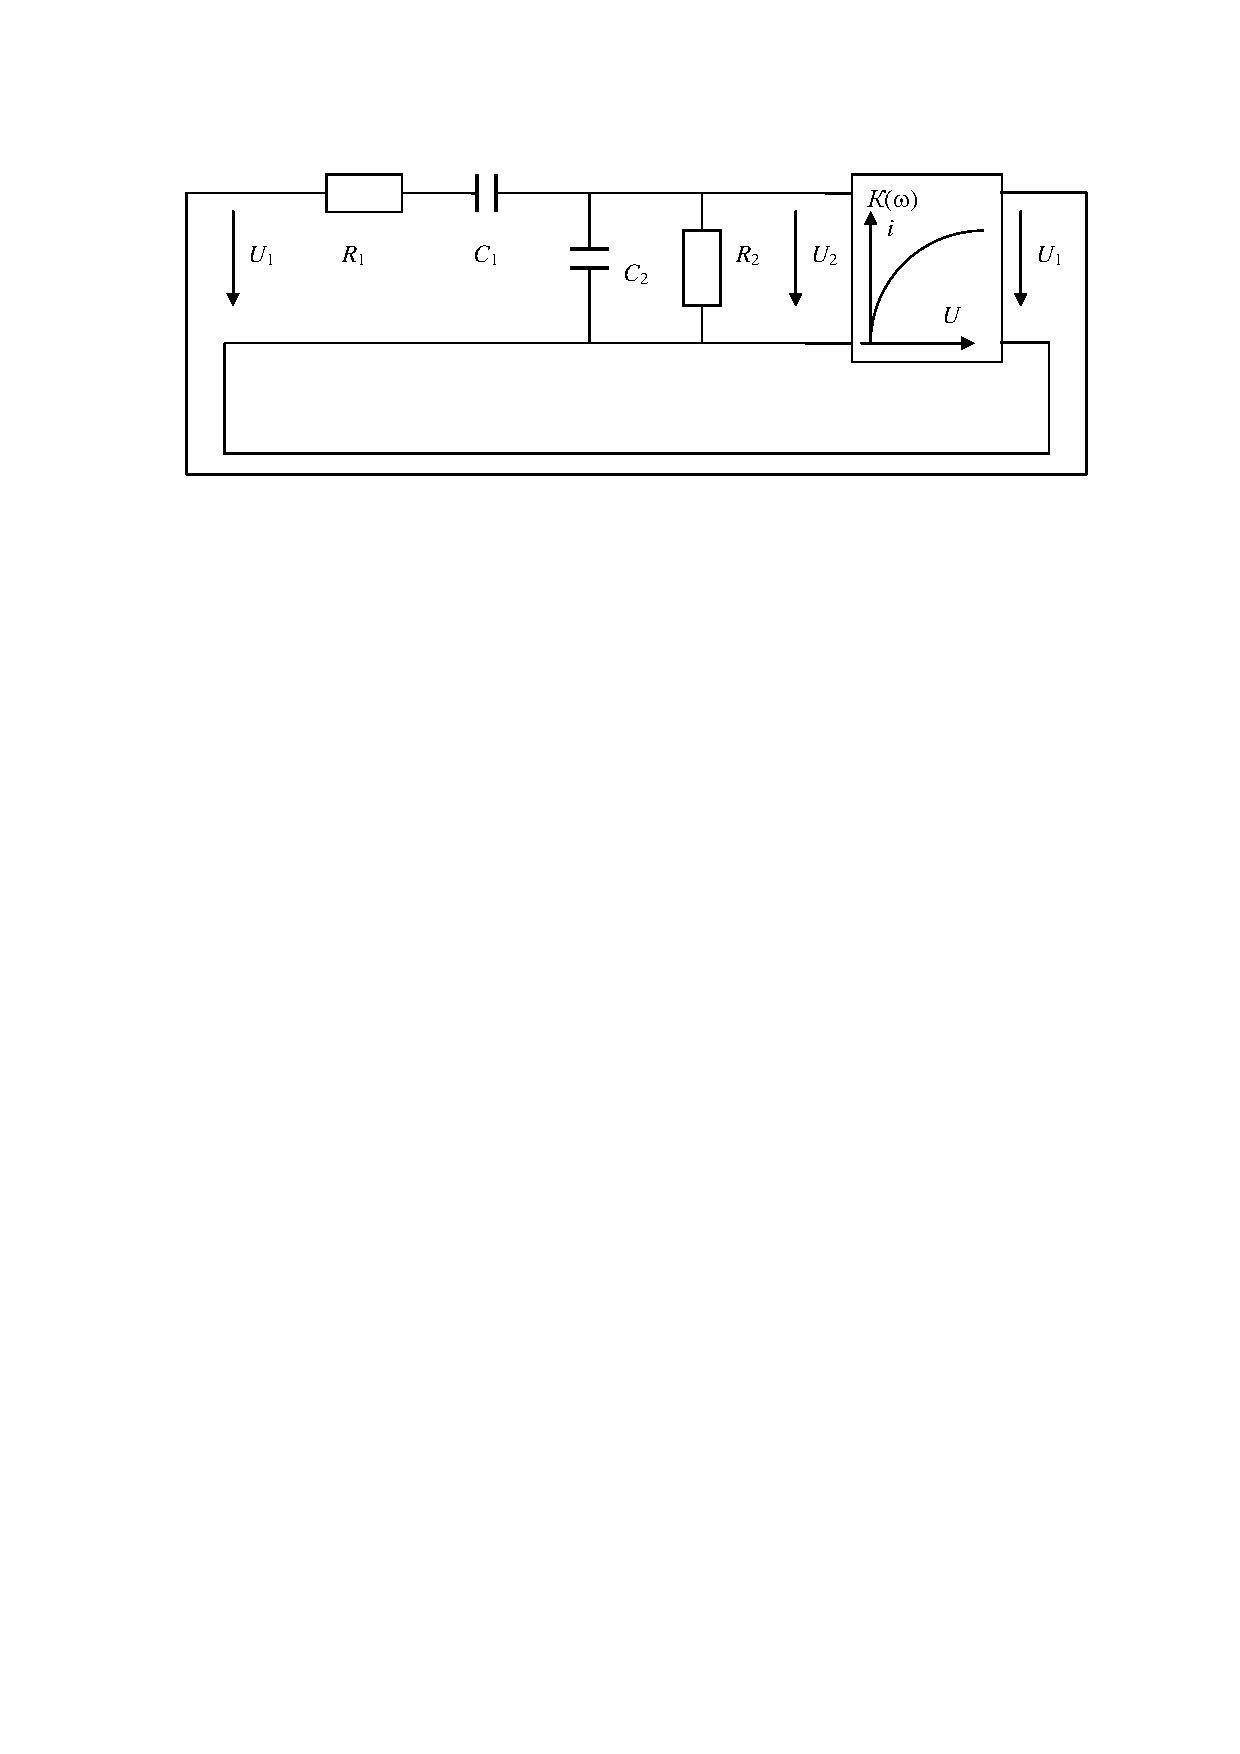
\includegraphics[]{fig/fig5-2.pdf}
	\caption{}
	\label{fig:5.2}
\end{figure}
Найдем дифференциальное уравнение схемы рис.  \ref{fig:5.2}, положив в ней $K(\omega)=\frac{U_1}{U_2}$, где $U_1$ -выходное напряжение усилителя $К(\omega)$, a $U_2$ -- входное. 
Из этого уравнения можно найти 
\begin{equation}
	U_1=K(\omega)\cdot U_2, \qquad
	\dv{U_1}{t}=K\dv{U_2}{t}.
\end{equation}
Подставляя полученное соотношение в \eqref{eq5.2}, получим
\begin{gather}
	\label{eq5.3}
	%
	\dv[2]{U_2}{t}+
		2 \alpha \dv{U_2}{t} -
		\frac{K}{\tau_{21}}	\dv{U_2}{t}+ 
		\omega_0^2 U_2 =
		0, 
	%
	\\ \text{или} \quad
	%
	\dv[2]{U_2}{t}+
		\qty(
			\frac{1}{\tau_1}+
			\frac{1}{\tau_2}+
			\frac{1-K}{\tau_{21}}
		)\dv{U_2}{t}+ 
		\omega_0^2 U_2=0, 
	\quad \text{где} \quad
	\tau_{21}=R_2C_1.
\end{gather}

Уравнение \eqref{eq5.3} совершенно аналогично уравнению \eqref{eq5.1} с $LC$-контуром. Для осуществления самовозбуждения необходимо сделать отрицательным коэффициент при первой производной
\begin{equation}
	\left(\frac{1}{R_{1} C_{1}}+\frac{1}{R_{2} C_{2}}+\frac{1-K}{R_{2} C_{1}}\right)<0
\end{equation}

Типичная схема RC-автогенератора приведена на рис.  \ref{fig:5.3}(а), а его эквивалентная схема с разомкнутой цепью обратной связи - на рис. \ref{fig:5.3}(б). Здесь $K_0$ - идеальный усилитель с вещественным и положительным коэффициентом усиления $K_0$. Выход усилителя соединяется с его входом через пассивный четырехполюсник, выделенный на рисунке пунктирной рамкой и представляющий собой цепь положительной обратной связи. Передаточная функция этой цепи равна
\begin{equation}
	\beta(j \omega)=
	\cfrac{
		\cfrac{
			R_{2}/{j \omega C_{2}}
		}{
			R_{2}+{1}/{j \omega C_{2}}}
	}{
		% \qty(
			R_1+\cfrac{1}{j \omega C_1}+
		% )+
		\cfrac{
			R_2/{j \omega C_2}
		}{
			R_2+1/{j \omega C_2}
		}
	}
\end{equation}
или в переменных Лапласа
\begin{gather}
 	\label{eq5.5}
	 \beta(p)=\frac{p \tau_{21}}{\left(1+p \tau_{1}\right)\left(1+p \tau_{2}\right)+p \tau_{21}}.
\end{gather}

Характеристическое уравнение автогенератора в общем виде имеет вид
\begin{gather}
	\label{eq5.6}
	K(j \omega) \beta(j \omega)-1=0 \qq{или} K(p) \beta(p)=1
\end{gather}
Для схемы рис. \ref{fig:5.3} с передаточной функцией цепи положительной обратной связи $\beta(p)$ в соответствии с \eqref{eq5.5} характеристическое уравнение имеет вид
\begin{gather}
	\label{eq5.7}
	a_{2} p^{2}+a_{1} p+1=0, \qq {где} a_{2}=\tau_{1} \tau_{2}, \quad a_{1}=\tau_{1}+\tau_{2}-\tau_{21}\left(K_{0}-1\right)
\end{gather}
\begin{figure}[H]
	\centering
	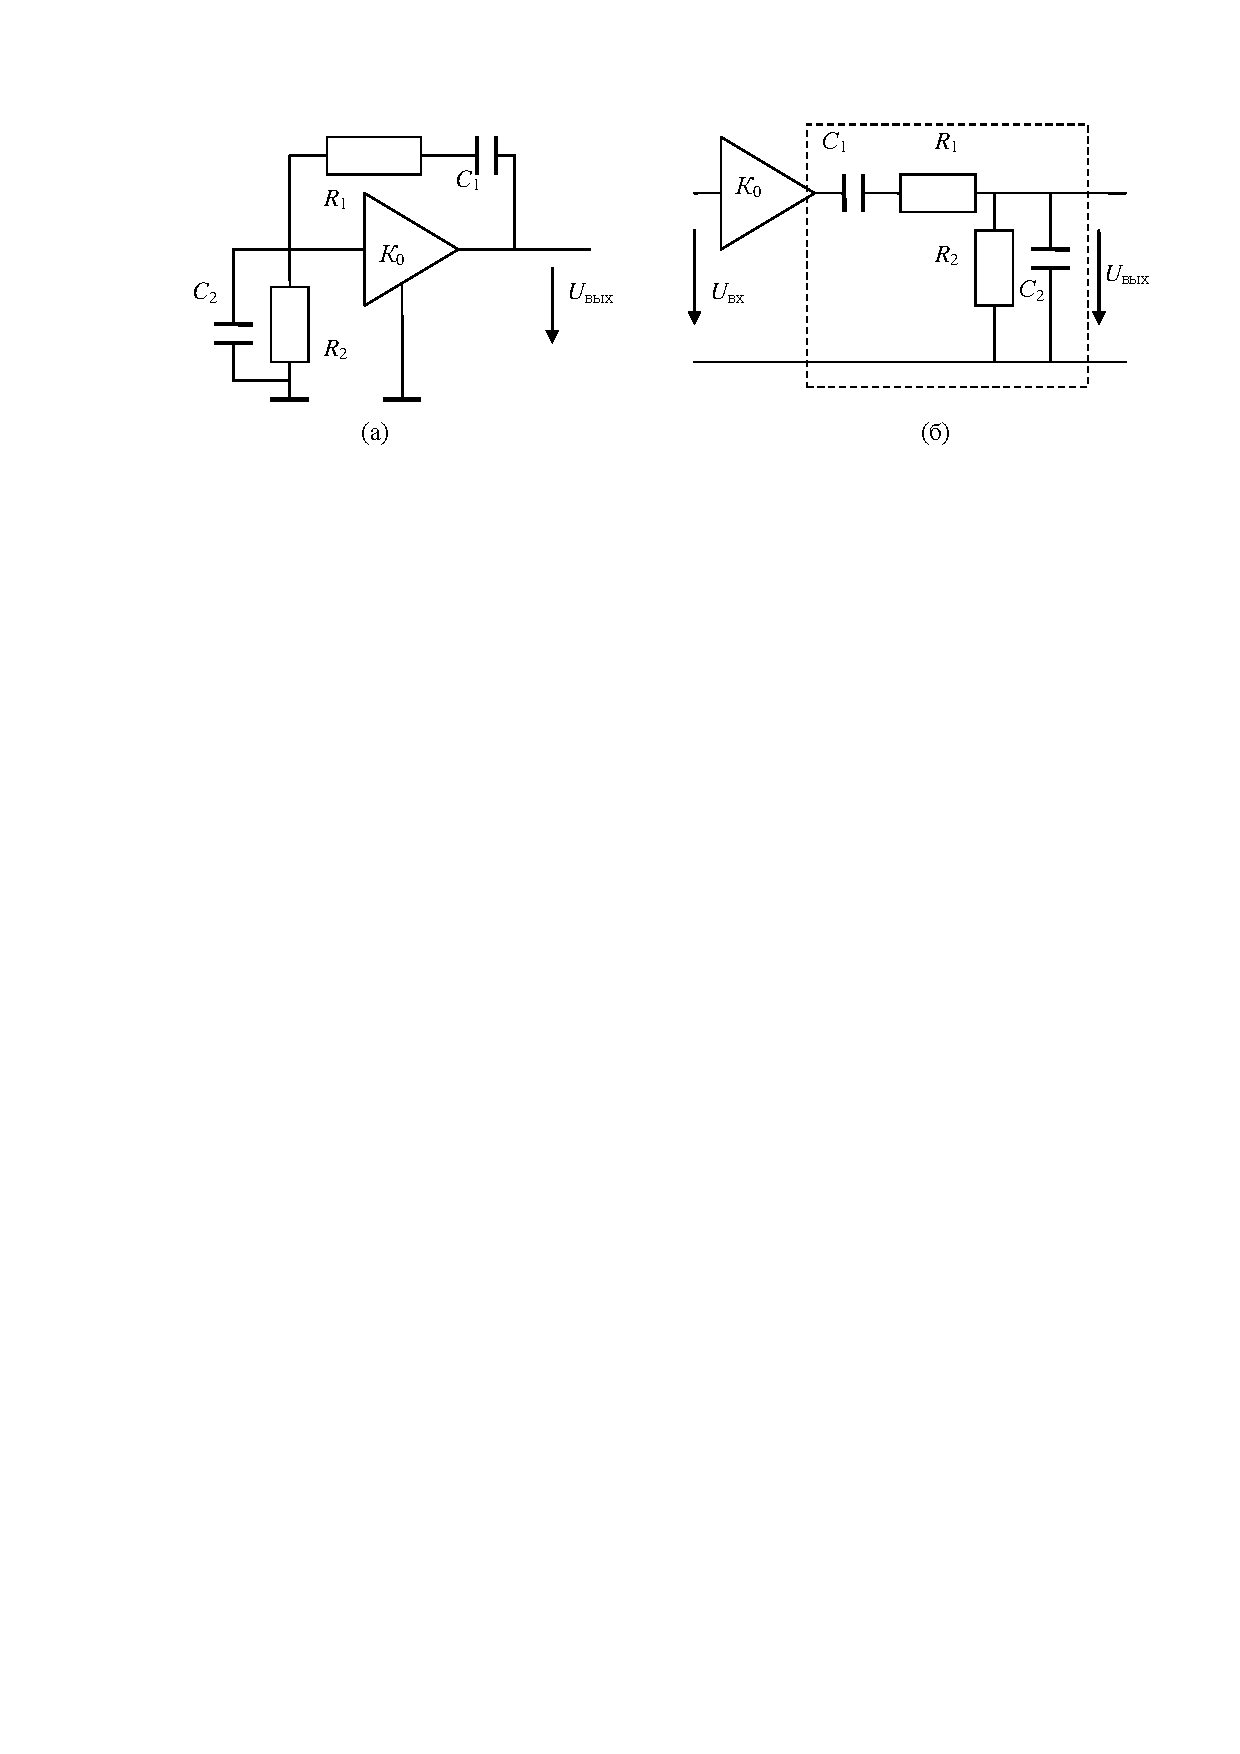
\includegraphics[]{fig/fig5-3.pdf}
	\caption{$RC$-генератор и его эквивалентная схема}
	\label{fig:5.3}
\end{figure}
Условия самовозбуждения автогенератора состоит в том, чтобы коэффициент $a_1$ был меньше нуля. Отсюда находится условие, налагаемое на коэффициент усиления $K_0$:
\begin{gather}
	\label{eq5.8}
	K_{0}>1+\frac{R_{1} C_{1}+R_{2} C_{2}}{R_{2} C_{1}}
\end{gather}
Частота генерации определяется мнимой частью корней характеристического уравнения \eqref{eq5.7}. Для стационарного режима автогенератора коэффициент $a_1$ этого уравнения равен нулю, и уравнение принимает вид
\begin{gather}
	\label{eq5.9}
	p^{2} \tau_{1} \tau_{2}+1=0.
\end{gather}
Мнимые части корней этого уравнения и частота генерации равны
\begin{gather}
	\label{eq5.10}
	p_{1,2}=\pm j \sqrt{\frac{1}{\tau_{1}\tau_{2}}}, \qquad
	\omega_{0}=\frac{1}{\sqrt{R_{1} R_{2} C_{1} C_{2}}}
\end{gather}
Обычно выбирают $R_{1}=R_{2}=R$ и $C_{1}=C_{2}=C$. При этом передаточная характеристика \eqref{eq5.5} принимает вид
\begin{gather}
	\label{eq5.11}
	\beta(j \omega)=\cfrac{
		j\qty[\cfrac{\omega}{\omega_0}]
	}{
		1+3j\qty[\cfrac{\omega}{\omega_0}]-
		\qty[\cfrac{\omega}{\omega_0}]^2
	}\,\,, \qq{где} 
	\omega_0=\frac{1}{RC}.
\end{gather}
Соответствующие амплитудно-частотная и фазо-частотная характеристики представлены на рис. \ref{fig:5.4} (а) и (б) соответственно.
\begin{figure}[H]
	\centering
	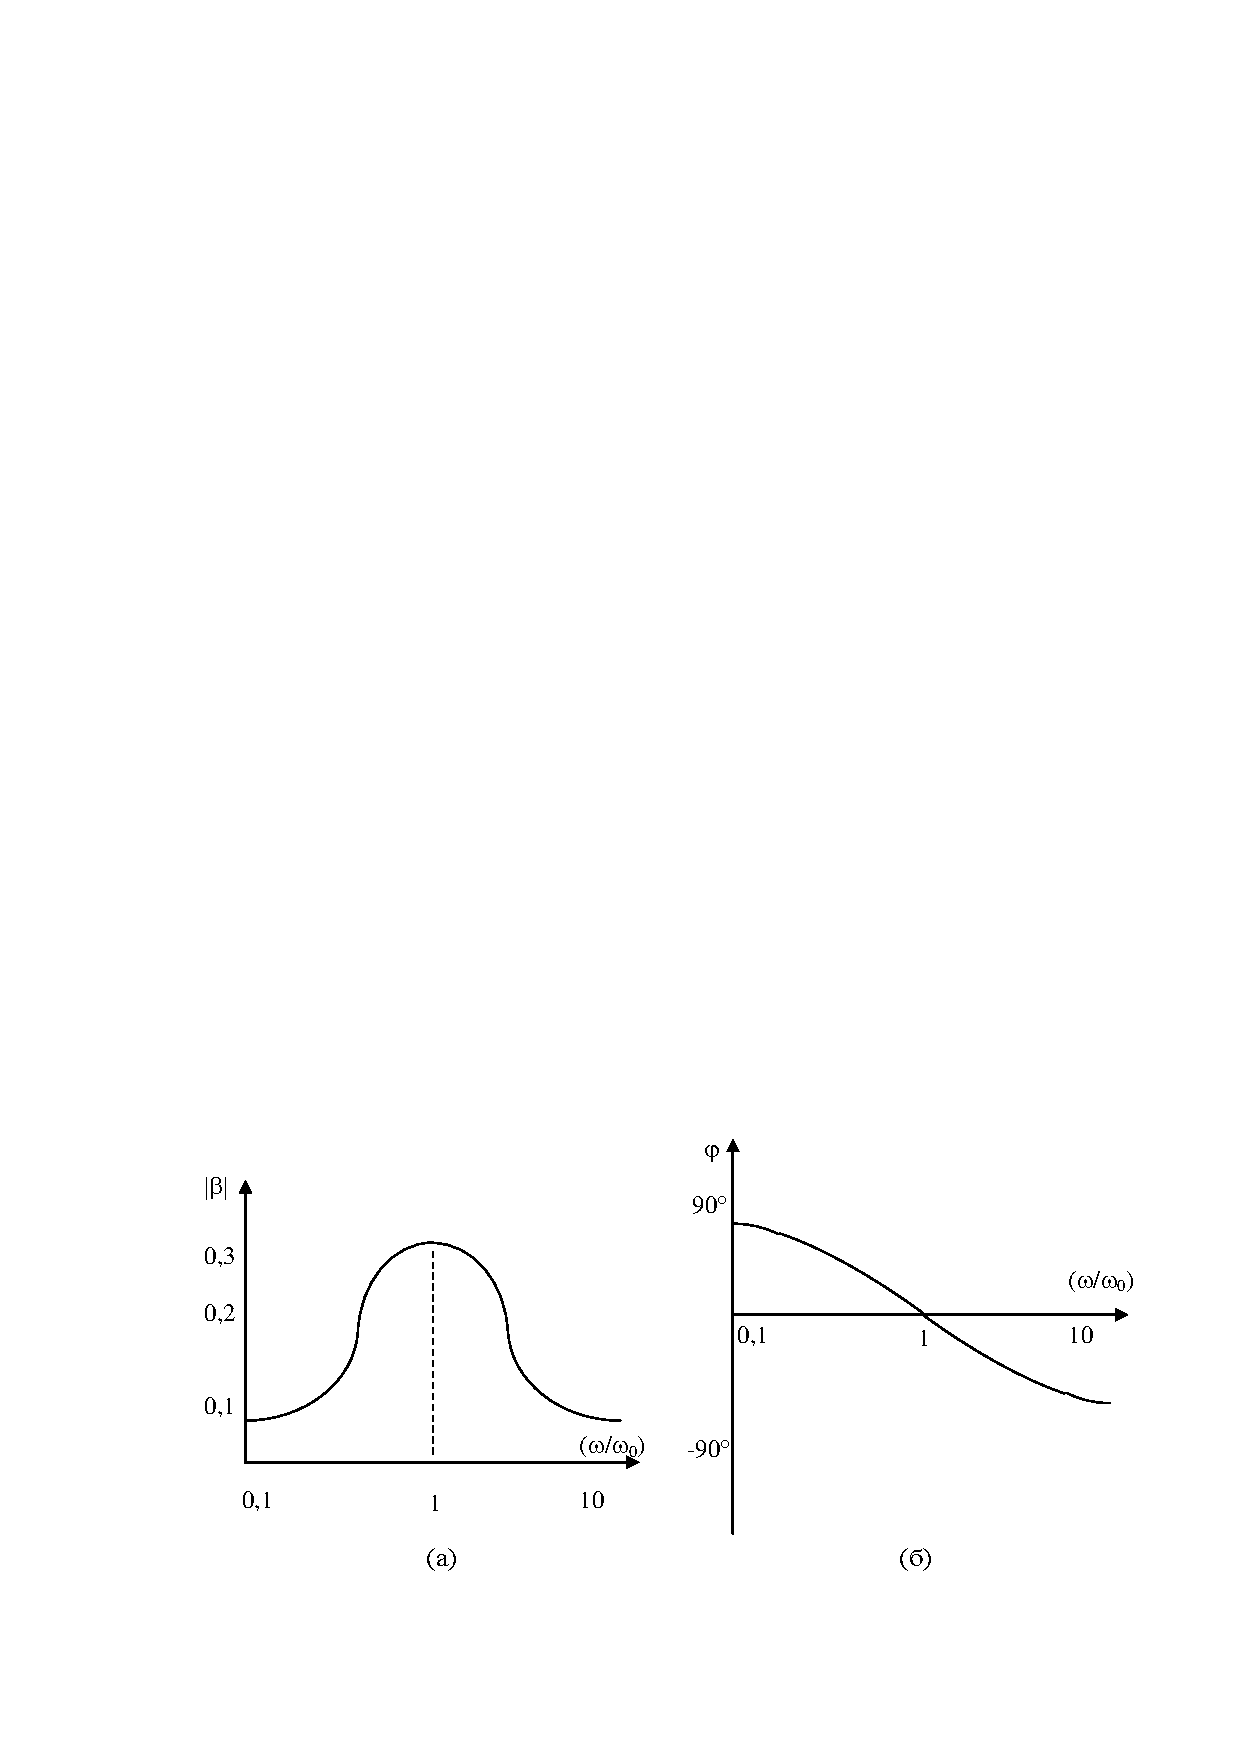
\includegraphics[]{fig/fig5-4.pdf}
	\caption{АЧХ и ФЧХ генератора}
	\label{fig:5.4}
\end{figure}
Условие возбуждения такого генератора на частоте $\omega_0$ при этом переходит в $K_0 > 3$. 

\section{Исследование частотного модулятора}
Мы займемся исследованием принципа действия частотного модулятора, получением характеристик частотного модулятора при воздействии на его вход гармонического сигнала (тональная модуляция) и исследование формы и спектра сигналов с частотной модуляцией.

\subsection{Схема работы и измерительная аппаратура}
В данной работе используется универсальный лабораторный стенд со сменным блоком <<частотный модем>>, упрощённая принципиальная схема которого приведена на рис. \ref{fig:6.1}. В первой части работы объектом исследования является левая часть схемы (между гнёздами КТ 1 и КТ 2).
\begin{figure}[H]
	\centering
	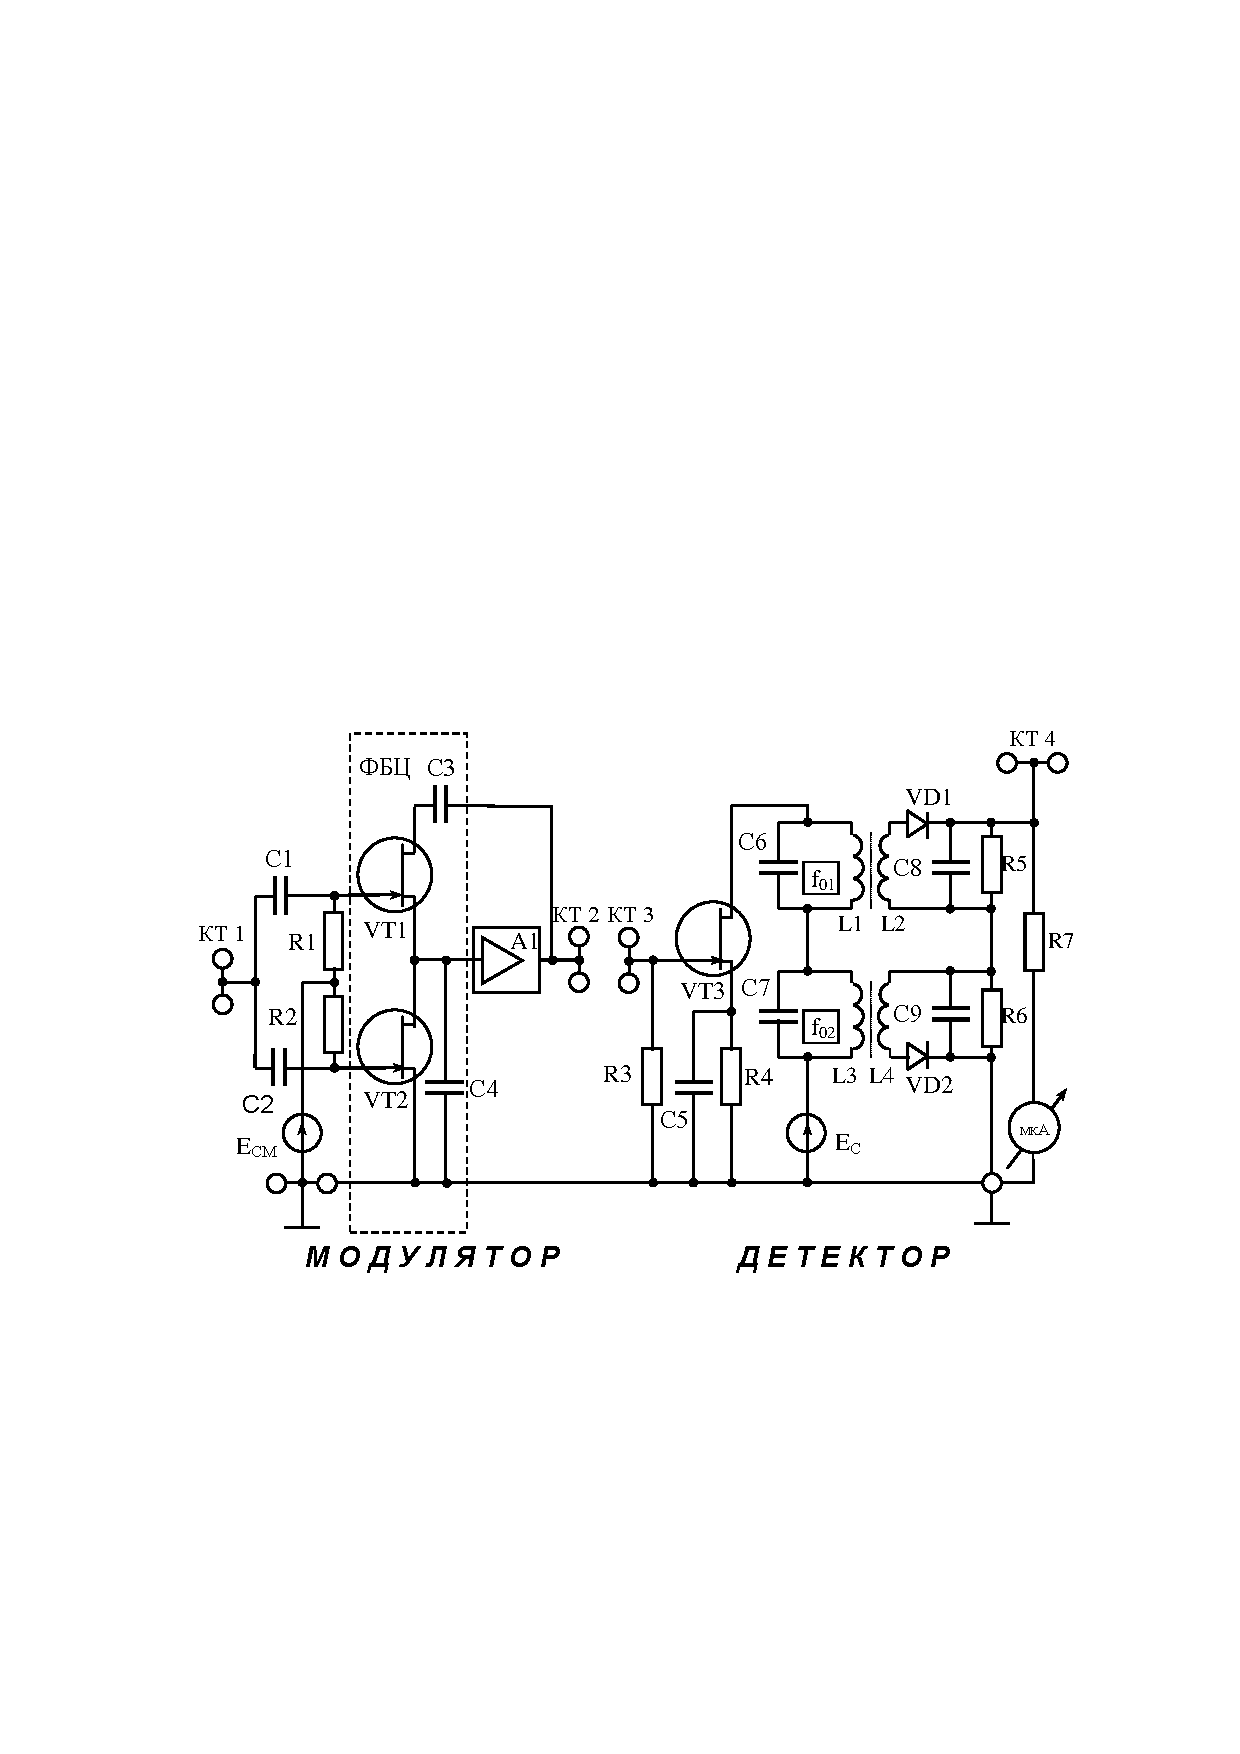
\includegraphics[scale=1]{fig/fig6-1}
	\caption{Упрощенная схема частотного модема}
	\label{fig:6.1}
\end{figure}

Частотный модулятор представляет собой $RC$-генератор, состоящий из двухкаскадного резистивного усилителя (А1) и фазобалансной цепи (ФБЦ), обеспечивающей положительную обратную связь. Частота генерации зависит от параметров ФБЦ - С3, С4 и сопротивлений каналов сток-исток полевых транзисторов VT1 и VT2. Сопротивление канала ($R_\text{си}$) зависит от управляющего напряжения, приложенного к затвору. Таким образом, полевой транзистор в ФБЦ является параметрическим элементом, управляемым модулирующим напряжением. Напряжение смещения ($E_\text{см}$), являющееся постоянной составляющей модулирующего сигнала, позволяет установить несущую частоту модулированного сигнала, а переменная составляющая, т.е. сам модулирующий сигнал, поданный на гнезда КТ 1, обеспечивает девиацию частоты $\Delta f_\text{max}$, зависящую от амплитуды модулирующего сигнала. Выходом частотного модулятора являются гнезда КТ 2.

В схеме модулятора имеется блок автоматической регулировки усиления, поддерживающий постоянную амплитуду ЧМ-сигнала (на схеме не показан).

В качестве источника модулирующего сигнала используется встроенный диапазонный генератор НЧ с цифровой индикацией частоты выходного гармонического сигнала, подключаемый к входу модулятора. Для контроля амплитуды модулирующего сигнала используется встроенный вольтметр. Измерение частот, анализ осциллограмм и спектра сигналов производится на двухлучевом цифровом осциллографе TDS 2002.

\section{Эксперимент}
\subsection{Измерение статической модуляционной характеристики}
Измерение СМХ: $f=\phi(E_\text{см})$ выполняется при отсутствии модулирующего сигнала. Последовательно изменяя значения $E_\text{см}$, определили значение частоты модулятора $f$.
\begin{figure}[!h]
	\centering
	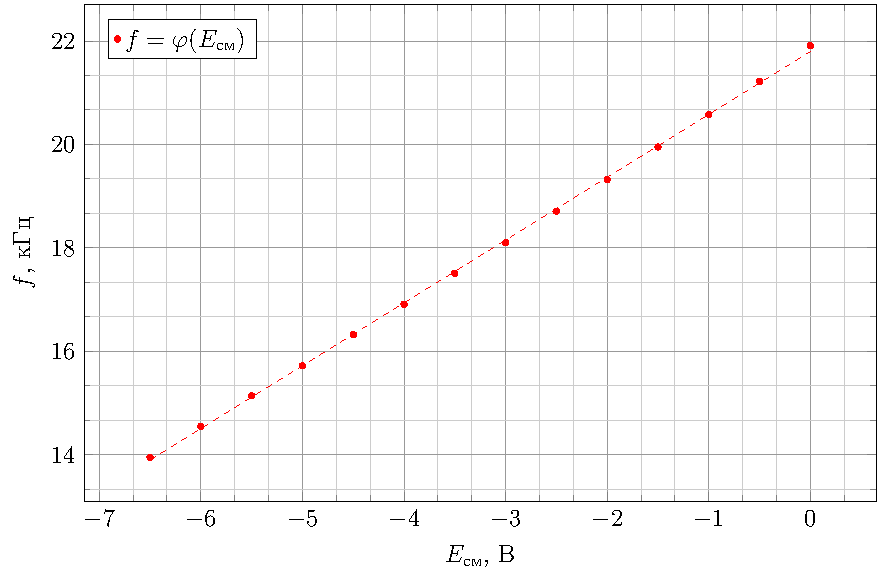
\includegraphics[scale=1]{plots/task1.pdf}
	\caption{СМХ}
	\label{fig:figure1}
\end{figure}
По полученным данным были определены:
\begin{enumerate}
	\item {Положение рабочей точки(середина линейного участка), из которой можно найти $E_\text{см опт}$ и $f_0$}
	\item {угол наклона линейного участка СМХ(тангенс этого угла соответствует коэффициенту $K_\text{чм}$ модулятора)}
	\item {границы линейного участка($f_{min},f_{max}$).}
\end{enumerate}
% Table generated by Excel2LaTeX from sheet 'задание1'
\begin{table}[htbp]
  \centering
  \caption{Параметры СМХ}
    \begin{tabular}{|r|r|r|r|r|}
    \toprule
    \multicolumn{1}{|l|}{$E_\text{см опт}$, В} & \multicolumn{1}{l|}{$f_0$, кГц} & \multicolumn{1}{l|}{$f_{min}$, кГц} & \multicolumn{1}{l|}{$f_{max}$, кГц} & \multicolumn{1}{l|}{$K_\text{чм}$, кГц/В} \\
    \midrule
    -3.5  & 17.51 & 13.95 & 21.91 & 1.2 \\
    \bottomrule
    \end{tabular}%
  \label{tab:tab1}%
\end{table}%
\subsection{Исследование влияния амплитуды модулирующего сигнала на спектр ЧМ}
По ряду заданных значений $M_\text{чм}$ рассчитали амплитуды модулирующих сигналов, а затем и действующие значения $U_c$, выбрав $F_\text{мод}=500\text{ Гц}$.
% Table generated by Excel2LaTeX from sheet 'задание2'
\begin{table}[htbp]
  \centering
  \caption{практическая ширина спектра в зависимости от коэффициента модуляции}
    \begin{tabular}{|l|r|r|r|r|r|r|}
    \toprule
    $M_\text{чм}$ & 0     & 0.1   & 0.5   & 1     & 2.4   & 3.8 \\
    \midrule
    $\Delta f_{max}$ & 0     & 50    & 250   & 500   & 1200  & 1900 \\
    \midrule
    $U_\text{мс}$ & 0.00  & 0.04  & 0.21  & 0.42  & 1.00  & 1.58 \\
    \midrule
    $U_\text{с}$  & 0.00  & 0.03  & 0.15  & 0.29  & 0.71  & 1.12 \\
    \midrule
    $2 \Delta f$ &       & 1000  & 1000  & 2000  & 3000  & 4000 \\
    \bottomrule
    \end{tabular}%
  \label{tab:tab2}%
\end{table}%
\begin{figure}[H]
	\centering
\begin{minipage}{0.45\linewidth}
	\centering
	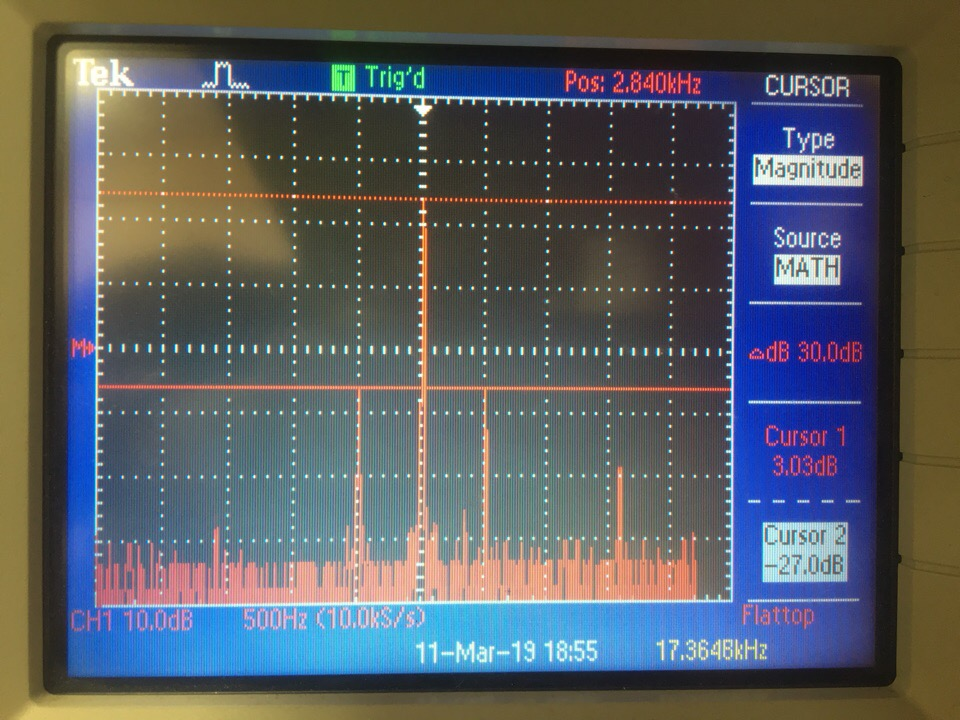
\includegraphics[width=\linewidth]{photo/task32(1).jpg}
\end{minipage}
\begin{minipage}{0.45\linewidth}
	\centering
	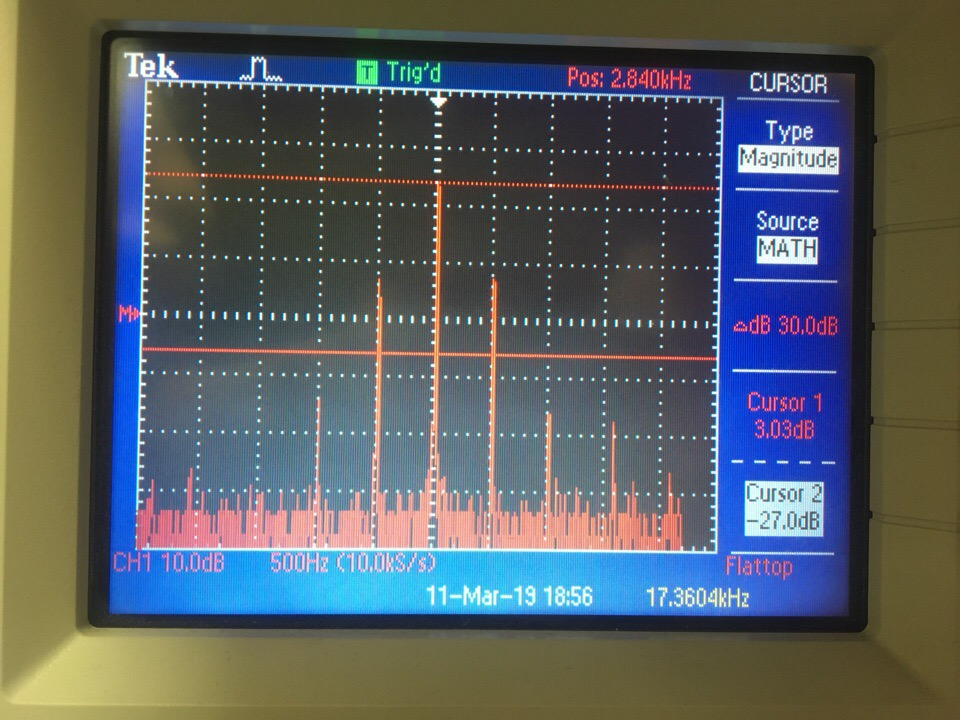
\includegraphics[width=\linewidth]{photo/task32(2).jpg}
\end{minipage}
\begin{minipage}{0.45\linewidth}
	\centering
	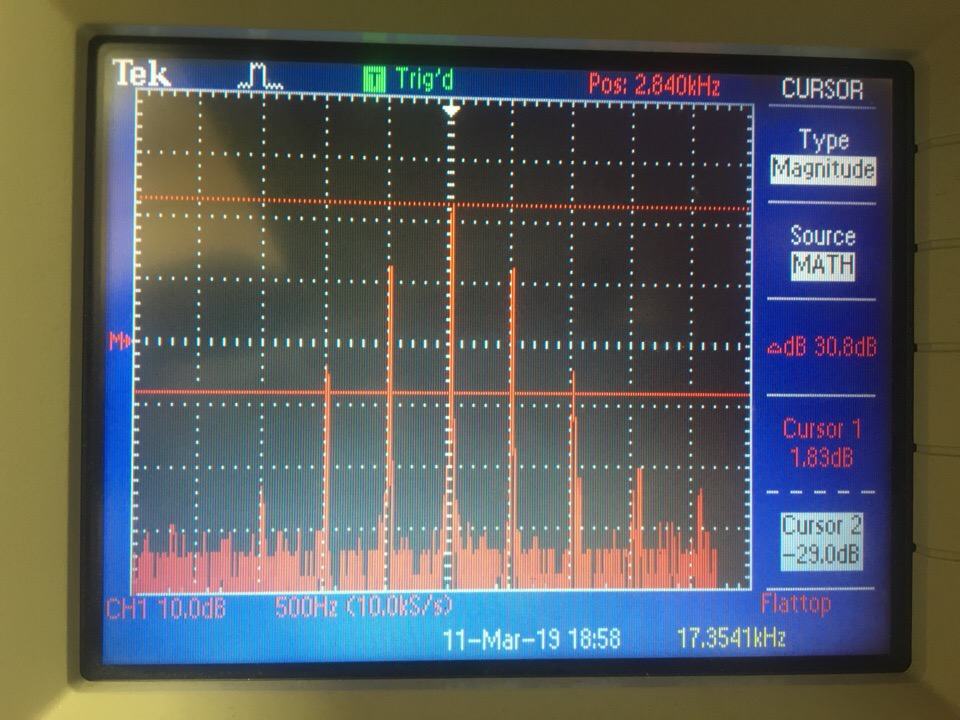
\includegraphics[width=\linewidth]{photo/task32(3).jpg}
\end{minipage}
\begin{minipage}{0.45\linewidth}
	\centering
	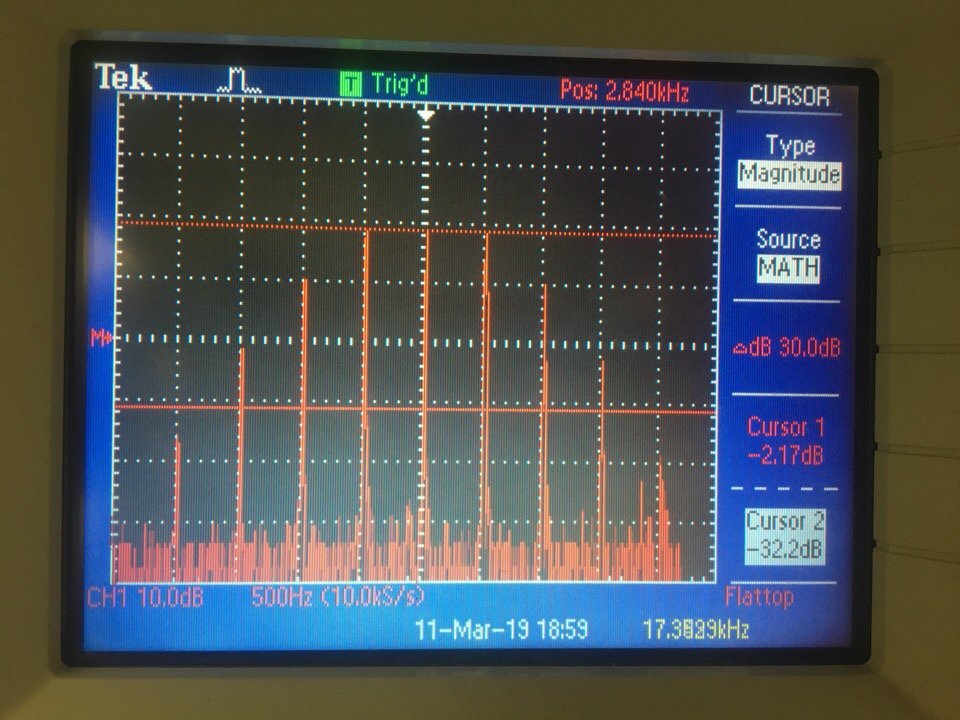
\includegraphics[width=\linewidth]{photo/task32(4).jpg}
\end{minipage}
\end{figure}
\begin{figure}
	\centering
	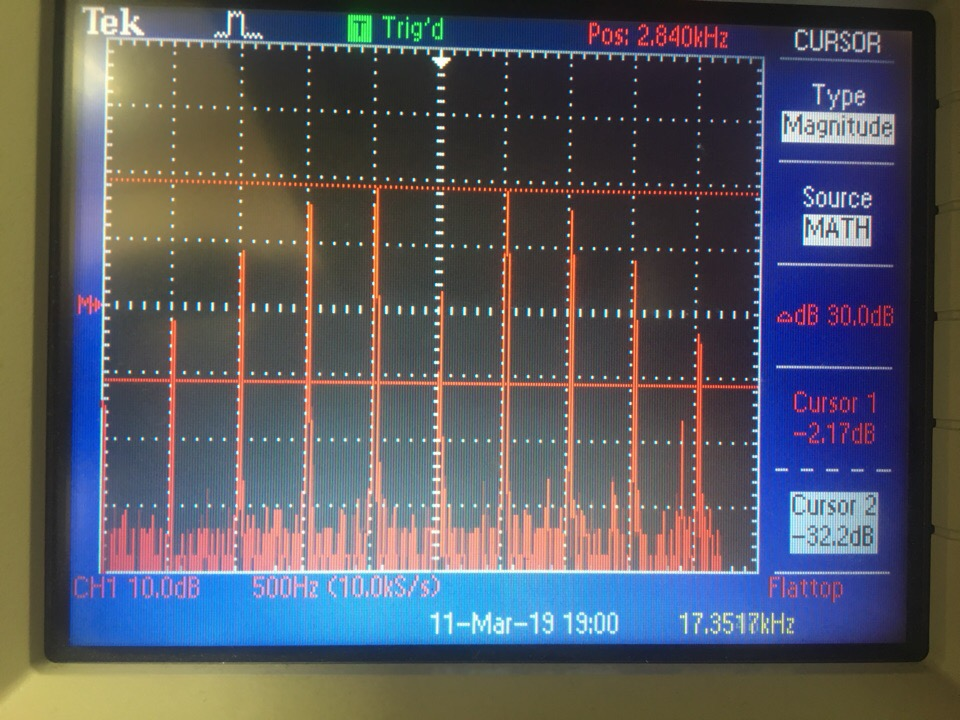
\includegraphics[width=0.45\linewidth]{photo/task32(5).jpg}
\end{figure}

\subsection{Исследование влияния частоты модуляции на спектр ЧМ-сигнала}
Зафиксировав амплитуду сигнала и несущую частоту ($U_\text{с}=0.707\text{ В}, f_0=17.51\text{ кГц}$), исследовали влияние частоты модуляции на ширину спектра.
% Table generated by Excel2LaTeX from sheet 'задание3'
\begin{table}[htbp]
  \centering
  \caption{Зависимость ширины спектра от частоты модуляции}
    \begin{tabular}{|l|r|r|r|r|r|}
    \toprule
    $F_\text{мод}$ & 50    & 100   & 250   & 500   & 1000 \\
    \midrule
    $2 \Delta f$ & 1800  & 1900  & 2000  & 2000  & 2000 \\
    \midrule
    $M_\text{чм}$ & 24    & 12    & 4.8   & 2.4   & 1.2 \\
    \bottomrule
    \end{tabular}%
  \label{tab:tab3}%
\end{table}%
\begin{figure}[H]
	\centering
	\begin{minipage}{0.4\linewidth}
		\centering
		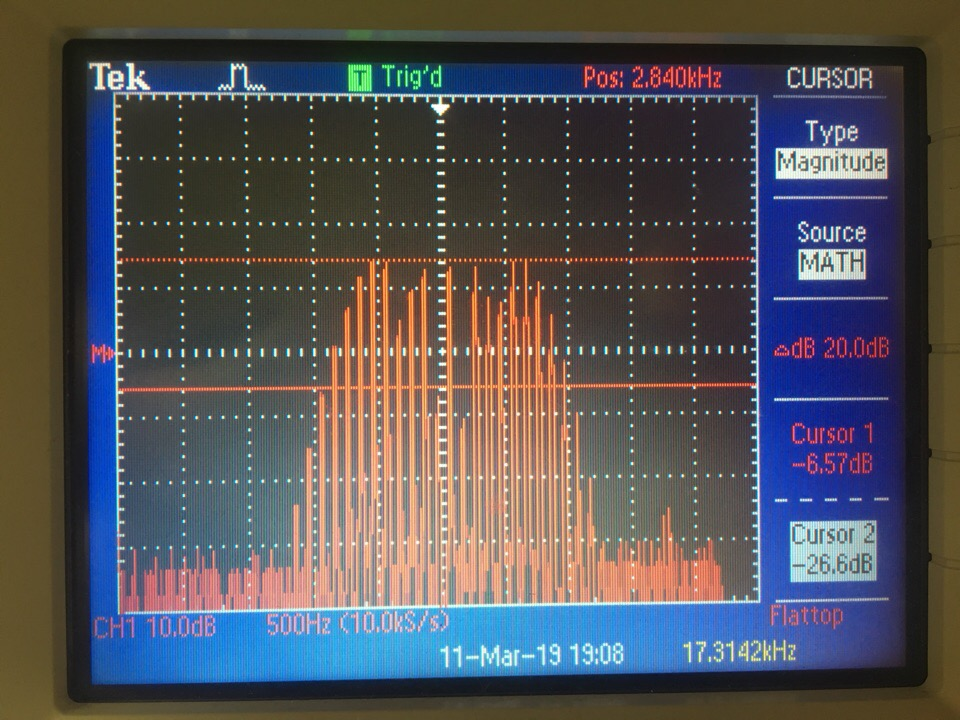
\includegraphics[width=\linewidth]{photo/task33(1).jpg}
	\end{minipage}
	\begin{minipage}{0.4\linewidth}
		\centering
		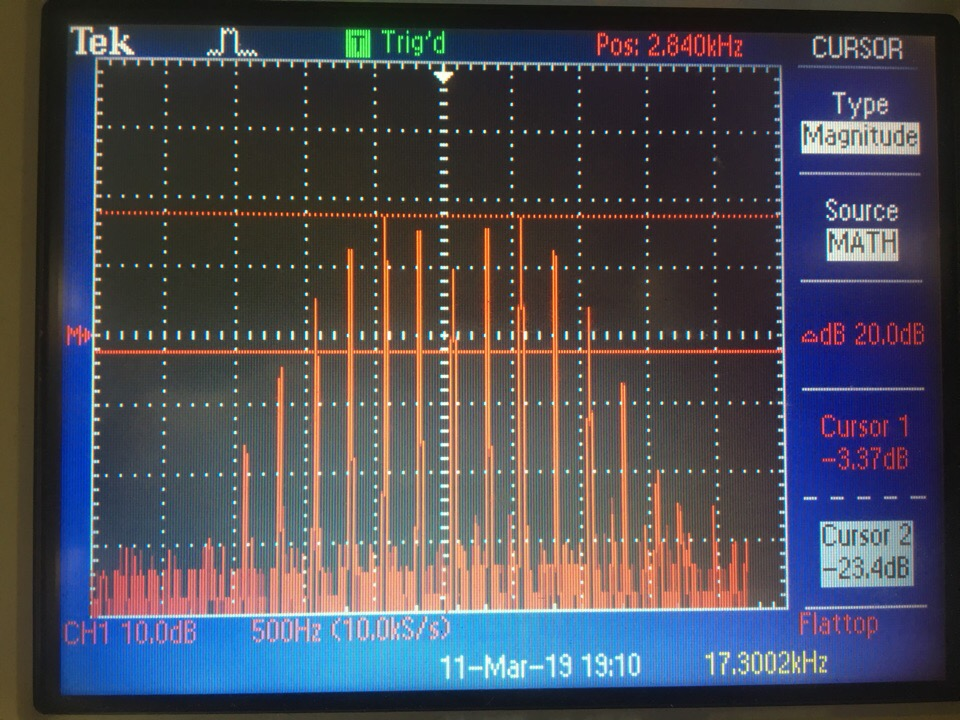
\includegraphics[width=\linewidth]{photo/task33(2).jpg}
	\end{minipage}
	\begin{minipage}{0.4\linewidth}
		\centering
		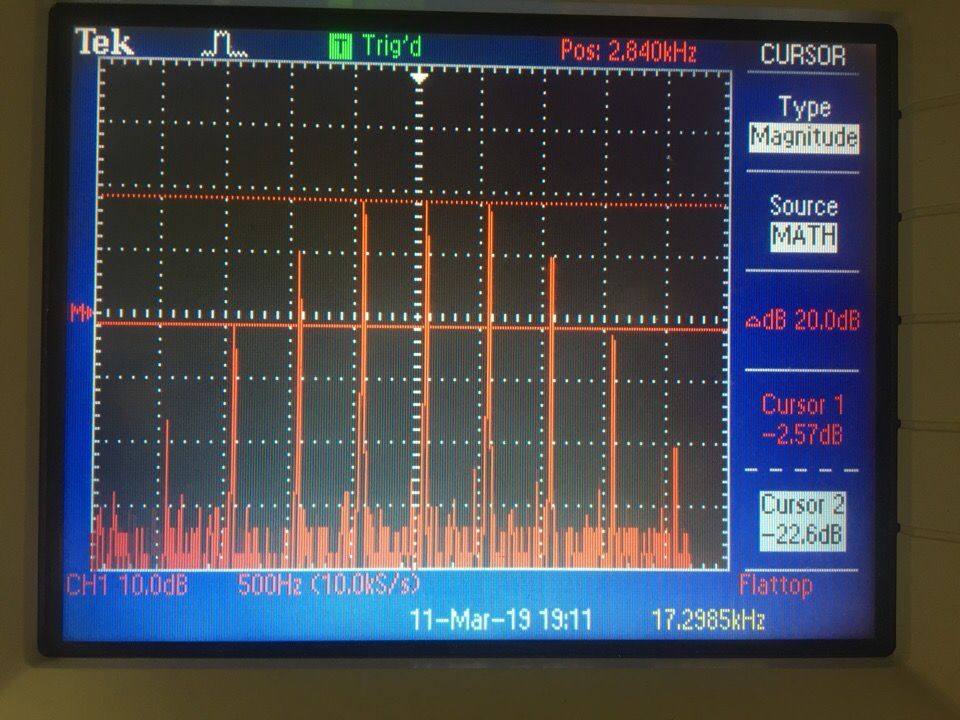
\includegraphics[width=\linewidth]{photo/task33(3).jpg}
	\end{minipage}
	\begin{minipage}{0.4\linewidth}
		\centering
		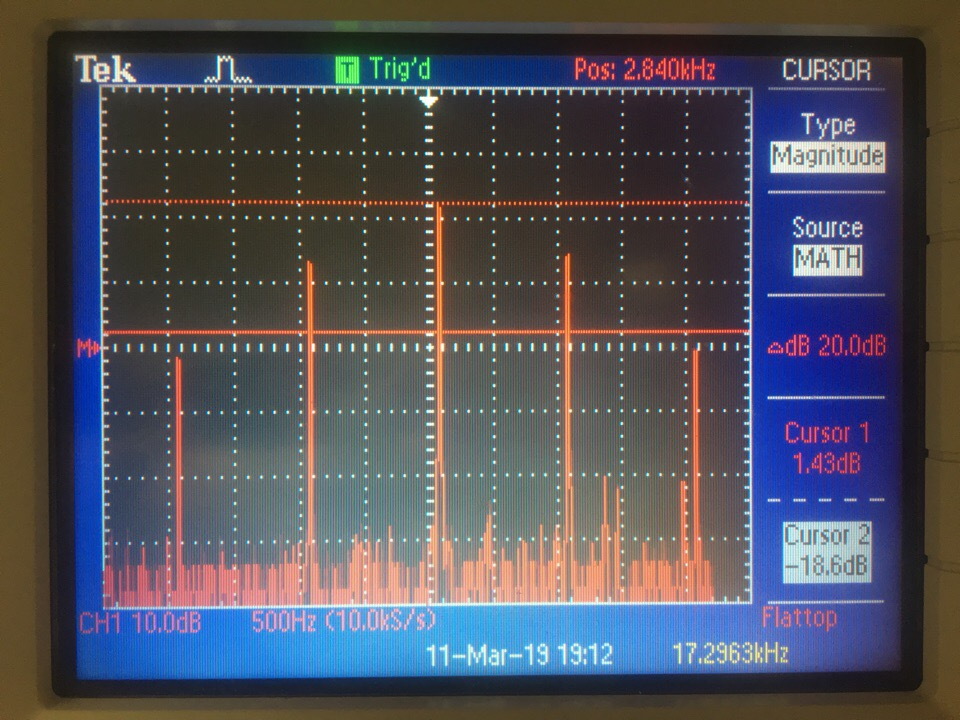
\includegraphics[width=\linewidth]{photo/task33(4).jpg}
	\end{minipage}
\end{figure}
\begin{figure}[H]
	\centering
	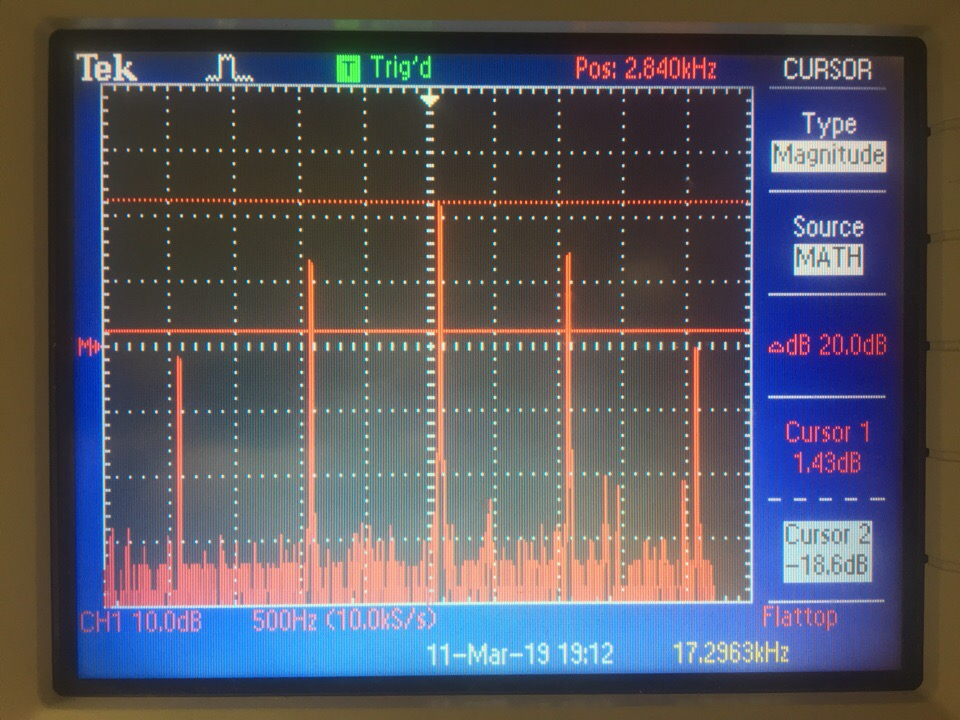
\includegraphics[width=0.45\linewidth]{photo/task33(5).jpg}
\end{figure}
\subsection{Исследование формы колебаний на входе и выходе частотного модулятора}
Зафиксировали осциллограммы на входе и выходе частотного модулятора. Оценили частоты выходного модулированного колебания на интервалах времени, соответствующих максимальному и минимальному уровням модулирующего колебания. Зафиксировали показания $1 / \Delta t$.
\begin{figure}[H]
	\centering
	\begin{minipage}{0.49\linewidth}
	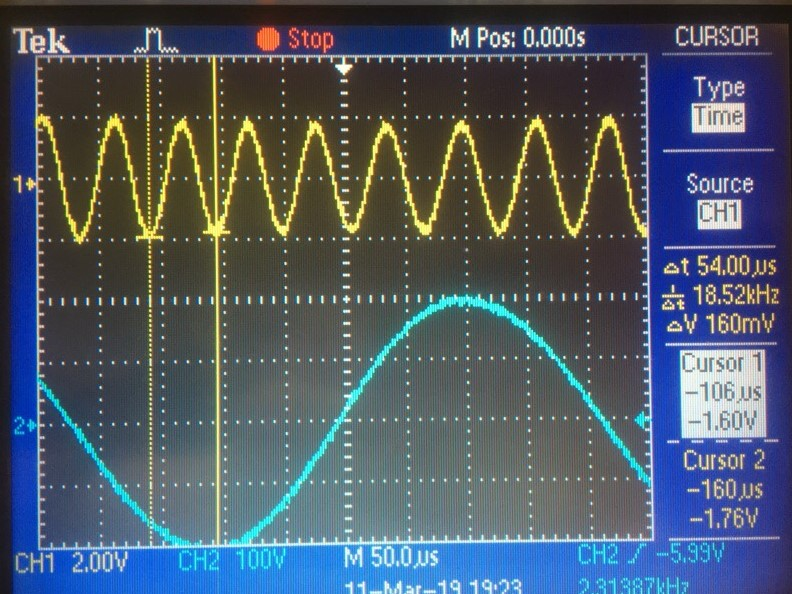
\includegraphics[width=\linewidth]{photo/task4(1).jpg}
	\end{minipage}
	\begin{minipage}{0.49\linewidth}
	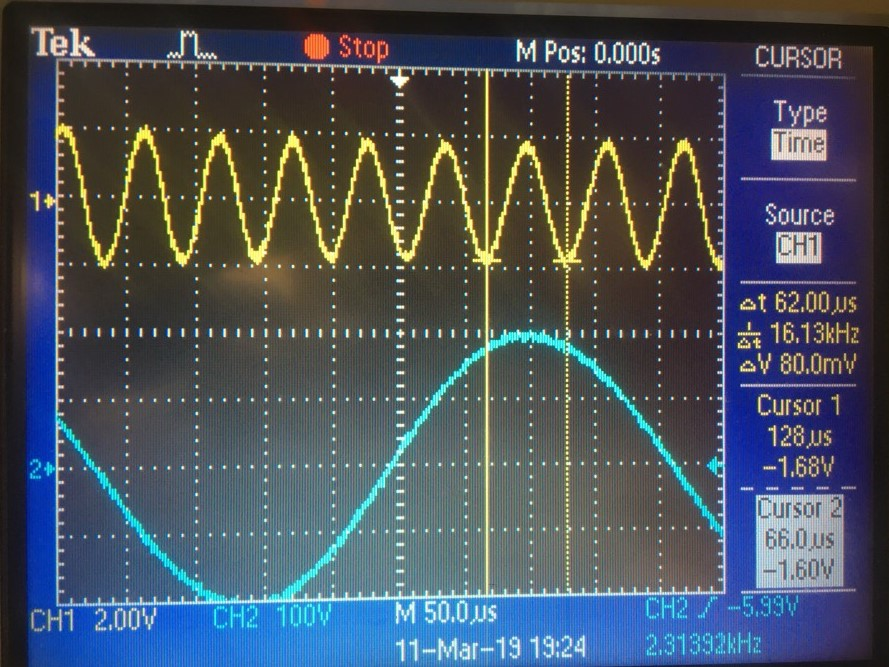
\includegraphics[width=\linewidth]{photo/task4(2).jpg}
	\end{minipage}
	\caption{}
	\label{fig:figure2}
\end{figure}
% Table generated by Excel2LaTeX from sheet 'задание4'
\begin{table}[htbp]
  \centering
  \caption{Зависимость частоты выходного сигнала от амплитуды модулирующего колебания}
    \begin{tabular}{|l|r|}
    \toprule
    $M_\text{чм}$     & \multicolumn{1}{l|}{$1/ \Delta t$, кГц} \\
    \midrule
    min   & 18.53 \\
    \midrule
    max   & 16.13 \\
    \bottomrule
    \end{tabular}%
  \label{tab:tab4}%
\end{table}%

\end{document}